\chapter{ZX Calculus} \label{ch:zx_calculus}

This chapter is a quick introduction to ZX calculus, a graphical calculus for quantum circuits.
Most parts of this chapter are based on the book \cite{KissingerWetering2024Book} and the lecture notes \cite{vandeweteringNotes}.

\section{Definition of ZX Calculus}

The theory of ZX calculus consists of two parts: the tensor network which is called ZX diagrams and the rewrite rules.
As ZX was invented to represent quantum circuits, all bonds in ZX diagrams are 2-dimensional.

ZX diagrams are generated by the following three classes of generators

\begin{definition}[Generators of ZX diagrams]
ZX diagrams have two classes of generators, $x$ and $z$ spiders, and one special tensor called the Hadamard gate.
\begin{enumerate}
	\item A rank-$k$ $z$-spider with phase $\phi$, which we denote as $z_{\phi}$, is a symmetric tensor such that $z_{\phi}(\underbrace{0, \cdots, 0}_{k}) = 1$, $z_{\phi}(1, 1, \cdots, 1) = \exp(i \phi)$, and all other entries are $0$.
	\item The Hadamard gate, denoted as $H$, is a 2-legged symmetric tensor that equals 
		\begin{equation}
			\frac{1}{\sqrt{2}}\begin{pmatrix}
				1 & 1 \\ 1 & -1
			\end{pmatrix}
		\end{equation} \label{eq:hadamard}
		 As a matrix, it is unitary and self-adjoint.
	\item A rank-$k$ $x$-spider with phase $\phi$, denoted as $x_{\phi}$, is a symmetric tensor that is the conjugation of $z_{\phi}$ of the same rank by the Hadamard gate.
\end{enumerate}
\end{definition}

These generators are shown in figure \ref{fig:zx_generators}. 
$z$-spiders are shown as green nodes, $x$-spiders red nodes, and their phases are shown as labels on the nodes. 
The Hadamard gate is shown as a yellow square.

\begin{figure}[ht]
	\centering
	% Graph Board TikZ export
% Exported: 2026-08-08T21:08:59.930Z
% Title: Untitled Graph
% Nodes: 28, Edges: 18

\begingroup
% --- Colors (define-if-not-already-defined) ---
\providecolor{zxRed}{RGB}{232,165,165}   % X spiders
\providecolor{zxGreen}{RGB}{216,248,216} % Z spiders
\providecolor{zxYellow}{RGB}{255,255,0}     % hadamard 

\tikzset{
    EMPTY/.style={minimum size=3.4mm,
        outer sep=-1.7mm},
    DOT/.style={inner sep=0mm, minimum size=3.4mm, shape=circle,
        draw=black, outer sep=-0.5mm, line width=1pt},
    BLACK_DOT/.style={minimum size=2mm,
        outer sep=-1mm, fill=black, shape=circle},
    WORD_BALL/.style={draw=black, shape=rectangle, minimum size=7.5mm,
        rounded corners=3.6mm, inner sep=1.2mm, outer sep=-0.5mm,
        scale=1, font={\Large\boldmath}, line width=1pt},
    GREEN_DOT/.style={DOT, fill=zxGreen},
    GREEN_WORD_BALL/.style={WORD_BALL, fill=zxGreen},
    RED_DOT/.style={DOT, fill=zxRed},
    RED_WORD_BALL/.style={GREEN_WORD_BALL, fill=zxRed},
    YELLOW_BOX/.style={fill=zxYellow, draw=black, line width=1pt, shape=rectangle, inner sep=0.6mm,
        minimum height=3.4mm, minimum width=3.4mm,
        font={\Large\boldmath}},
    EDGE/.style={draw=black, line width=1pt}
}
\pgfdeclarelayer{edgelayer}
\pgfdeclarelayer{nodelayer}
\pgfsetlayers{edgelayer,nodelayer,main}

\begin{tikzpicture}
    \begin{pgfonlayer}{nodelayer}
        \node [GREEN_WORD_BALL] (1) at (-3.07143, 0.21429) {$\alpha$};
        \node [EMPTY] (2) at (-4.57143, 1.21429) {};
        \node [EMPTY] (3) at (-4.57143, 0.71429) {};
        \node [EMPTY] (4) at (-4.57143, -0.28571) {};
        \node [EMPTY] (5) at (-4.57143, -0.78571) {};
        \node [EMPTY] (6) at (-4.57143, 0.21429) {$\cdots$};
        \node [EMPTY] (7) at (-1.57143, 1.21429) {};
        \node [EMPTY] (8) at (-1.57143, 0.71429) {};
        \node [EMPTY] (9) at (-1.57143, -0.28571) {};
        \node [EMPTY] (10) at (-1.57143, -0.78571) {};
        \node [EMPTY] (11) at (-1.57143, 0.21429) {$\cdots$};
        \node [RED_WORD_BALL] (12) at (1.42857, 0.21429) {$\alpha$};
        \node [EMPTY] (13) at (-0.07143, 1.21429) {};
        \node [EMPTY] (14) at (-0.07143, 0.71429) {};
        \node [EMPTY] (15) at (-0.07143, -0.28571) {};
        \node [EMPTY] (16) at (-0.07143, -0.78571) {};
        \node [EMPTY] (17) at (-0.07143, 0.21429) {$\cdots$};
        \node [EMPTY] (18) at (2.92857, 1.21429) {};
        \node [EMPTY] (19) at (2.92857, 0.71429) {};
        \node [EMPTY] (20) at (2.92857, -0.28571) {};
        \node [EMPTY] (21) at (2.92857, -0.78571) {};
        \node [EMPTY] (22) at (2.92857, 0.21429) {$\cdots$};
        \node [EMPTY] (23) at (4.92857, 1.21429) {};
        \node [EMPTY] (24) at (4.92857, -0.78571) {};
        \node [YELLOW_BOX] (25) at (4.92857, 0.21429) {};
        \node [label=above:{$z \text{ spider}$}, EMPTY] (26) at (-3.07143, -1.78571) {};
        \node [label=above:{$x \text{ spider}$}, EMPTY] (27) at (1.42857, -1.78571) {};
        \node [label=above:{$\text{Hadamard}$}, EMPTY] (28) at (4.92857, -1.78571) {};
    \end{pgfonlayer}
    \begin{pgfonlayer}{edgelayer}
        \draw[EDGE] (1) to (4);
        \draw[EDGE] (5) to (1);
        \draw[EDGE] (2) to (1);
        \draw[EDGE] (3) to (1);
        \draw[EDGE] (7) to (1);
        \draw[EDGE] (8) to (1);
        \draw[EDGE] (9) to (1);
        \draw[EDGE] (10) to (1);
        \draw[EDGE] (12) to (15);
        \draw[EDGE] (16) to (12);
        \draw[EDGE] (13) to (12);
        \draw[EDGE] (14) to (12);
        \draw[EDGE] (18) to (12);
        \draw[EDGE] (19) to (12);
        \draw[EDGE] (20) to (12);
        \draw[EDGE] (21) to (12);
        \draw[EDGE] (23) to (25);
        \draw[EDGE] (25) to (24);
    \end{pgfonlayer}
\end{tikzpicture}

\endgroup
	\caption{Generators of ZX diagrams.}
	\label{fig:zx_generators}
\end{figure}

Since ZX calculus was invented to represent quantum circuits, most authors treat them as linear maps with an input and an output instead of a generic tensor.
Following the conventional bra-ket notation where $\ket{a}$ denotes a state (a vector, usually written in column) and $\bra{a}$ denotes its dual (co-vector, also called an effect, written in row), $z$, $x$ and $H$ nodes can be represented in the following ways
\begin{align*}
	z_{\phi} &= \ket{0}^{\otimes n}\bra{0}^{\otimes m} + e^{i \phi} \ket{1}^{\otimes n}\bra{1}^{\otimes m} \\
	H &=\frac{1}{\sqrt{2}}(\ket{0}\bra{0} + \ket{0}\bra{1} + \ket{1}\bra{0} - \ket{1}\bra{1}) \\
	x_{\phi} &=  \ket{+}^{\otimes n}\bra{+}^{\otimes m} + e^{i \phi} \ket{-}^{\otimes n}\bra{-}^{\otimes m}
\end{align*}
where $\ket{+}$ and $\ket{-}$ denote the orthonormal basis $\frac{1}{\sqrt{2}}(\ket{0} + \ket{1})$ and $\frac{1}{\sqrt{2}}(\ket{0} - \ket{1})$ respectively.
Note that $H\ket{+} = \ket{0}$, $H\ket{-} = \ket{1}$, and $HH = I$.

The second part of ZX calculus is its rewrite rules,
which are the statements that certain combinations of generators are equivalent to each other.
Two ZX diagrams are equivalent if they represent the same tensor or they represent the same tensor up to a global constant. (This is because in quantum computation a global constant does not change the result quantum measurement.)
Throughout this dissertation, a strict equality will be denoted by a $=$ sign, while an equality up to a global constant will be denoted by a $\propto$ sign. \footnote{In the literature of ZX calculus, often the equal $=$ sign denotes both strict equality and equality up to a global constant.}
There are infinitely many rewrite rules, but the following are the most crucial ones.
\begin{definition}[Rewrite rules of ZX diagrams]
	Eight of the most important rewrite rules are shown in figure \ref{fig:zx_rewrites} and explained as follows:
	\begin{enumerate}
	\item Spider fusion, denoted as $\color{red} \mathbf{f}$. 
		A ZX diagram consisting only of $z$-spiders is equivalent to a single $z$-spider with the sum of the phases of the original spiders as its phase.
	\item color change, denoted as $\color{red} \mathbf{c}$.
		A $z$-spider with phase $\phi$ is equivalent to an $x$-spider with phase $\phi$ conjugated by Hadamard gates on all its legs.
	\item Hadamard cancellation, denoted as $\color{red} \mathbf{hh}$.
	\item Identity removal, denoted as $\color{red} \mathbf{id}$.
		A single rank-2 $z$-spider with phase $0$ and one input and one output leg is equivalent to the identity (a single bond).
		Two Hadamard gates are equivalent to the identity.
	\item $\pi$-copy, denoted as $\color{red} \mathbf{p}$. A $\pi$-phase $x$-spider can be copied through a $z$-spider, and vice versa.
	\item Copy rule, denoted as $\color{red} \mathbf{cp}$. A $0$-phase $x$-spider can be copied through a $z$-spider.
	\item Strong complementarity, denoted as $\color{red} \mathbf{sc}$. 
		Two sets of 0-phased $z$ and $x$ spiders that form a complete bipartite graph can be transformed into a simpler graph where the set of $z$ spiders are replaced with the same ranked $x$-spider, and the set of $x$-spiders are replaced with the same ranked $z$-spider.
		This is the most \emph{crucial} one for our later discussion. 
	\item Euler decomposition, denoted as $\color{red} \mathbf{e}$. 
		Hadamard gate can be decomposed into a sequence of $z$ and $x$ spiders with specific phases following the Euler decomposition of single qubit unitaries.
\end{enumerate}

\begin{figure}[ht]
	\centering
	\resizebox{\linewidth}{!}{
		% Graph Board TikZ export
% Exported: 2026-08-09T17:21:23.093Z
% Title: Untitled Graph
% Nodes: 111, Edges: 72

\begingroup
% --- Colors (define-if-not-already-defined) ---
\providecolor{zxRed}{RGB}{232,165,165}   % X spiders
\providecolor{zxGreen}{RGB}{216,248,216} % Z spiders
\providecolor{zxYellow}{RGB}{255,255,0}     % hadamard 

\tikzset{
    EMPTY/.style={minimum size=3.4mm,
        outer sep=-1.7mm},
    DOT/.style={inner sep=0mm, minimum size=3.4mm, shape=circle,
        draw=black, outer sep=-0.5mm, line width=1pt},
    BLACK_DOT/.style={minimum size=2mm,
        outer sep=-1mm, fill=black, shape=circle},
    WORD_BALL/.style={draw=black, shape=rectangle, minimum size=6.5mm,
        rounded corners=3.2mm, inner sep=1.2mm, outer sep=-1.0mm,
        scale=1, font={\large\boldmath}, line width=1pt},
    GREEN_DOT/.style={DOT, fill=zxGreen},
    GREEN_WORD_BALL/.style={WORD_BALL, fill=zxGreen},
    RED_DOT/.style={DOT, fill=zxRed},
    RED_WORD_BALL/.style={GREEN_WORD_BALL, fill=zxRed},
    YELLOW_BOX/.style={fill=zxYellow, draw=black, line width=1pt, shape=rectangle, inner sep=0.6mm,
        minimum height=3.4mm, minimum width=3.4mm,
        font={\large\boldmath}},
    EDGE/.style={draw=black, line width=1pt}
}
\pgfdeclarelayer{edgelayer}
\pgfdeclarelayer{nodelayer}
\pgfsetlayers{edgelayer,nodelayer,main}

\begin{tikzpicture}
    \begin{pgfonlayer}{nodelayer}
        \node [GREEN_WORD_BALL] (1) at (-7.29636, 3.29974) {$\alpha$};
        \node [GREEN_WORD_BALL] (2) at (-6.29636, 2.29974) {$\beta$};
        \node [EMPTY] (3) at (-7.29636, 2.79974) {};
        \node [EMPTY] (4) at (-6.29636, 2.79974) {};
        \node [EMPTY] (5) at (-6.79636, 2.79974) {$\cdots$};
        \node [EMPTY] (6) at (-8.29636, 4.29974) {};
        \node [EMPTY] (7) at (-8.29636, 3.29974) {};
        \node [EMPTY] (8) at (-8.29636, 2.29974) {};
        \node [EMPTY] (9) at (-8.29636, 1.29974) {};
        \node [EMPTY] (10) at (-5.29636, 4.29974) {};
        \node [EMPTY] (11) at (-5.29636, 3.29974) {};
        \node [EMPTY] (12) at (-5.29636, 2.29974) {};
        \node [EMPTY] (13) at (-5.29636, 1.29974) {};
        \node [EMPTY] (14) at (-5.29636, 3.79974) {$\cdots$};
        \node [EMPTY] (15) at (-5.29636, 1.79974) {$\cdots$};
        \node [EMPTY] (16) at (-8.29636, 1.79974) {$\cdots$};
        \node [EMPTY] (17) at (-8.29636, 3.79974) {$\cdots$};
        \node [label=above:{$\color{red} \mathbf{f}$}, EMPTY] (18) at (-3.79636, 2.79974) {$=$};
        \node [GREEN_WORD_BALL] (19) at (-0.79636, 2.79974) {$\alpha+\beta$};
        \node [EMPTY] (20) at (-2.29636, 4.29974) {};
        \node [EMPTY] (21) at (-2.29636, 3.29974) {};
        \node [EMPTY] (22) at (-2.29636, 2.29974) {};
        \node [EMPTY] (23) at (-2.29636, 1.29974) {};
        \node [EMPTY] (24) at (0.70364, 4.29974) {};
        \node [EMPTY] (25) at (0.70364, 3.29974) {};
        \node [EMPTY] (26) at (0.70364, 2.29974) {};
        \node [EMPTY] (27) at (0.70364, 1.29974) {};
        \node [EMPTY] (28) at (0.70364, 3.79974) {$\cdots$};
        \node [EMPTY] (29) at (0.20364, 1.79974) {$\cdots$};
        \node [EMPTY] (30) at (-2.29636, 1.79974) {$\cdots$};
        \node [EMPTY] (31) at (-2.29636, 3.79974) {$\cdots$};
        \node [GREEN_WORD_BALL] (32) at (4.27656, 3.03932) {$\alpha$};
        \node [YELLOW_BOX] (33) at (3.27656, 4.03932) {};
        \node [YELLOW_BOX] (34) at (3.27656, 2.03932) {};
        \node [YELLOW_BOX] (35) at (5.27656, 4.03932) {};
        \node [YELLOW_BOX] (36) at (5.27656, 2.03932) {};
        \node [EMPTY] (37) at (6.27656, 3.03932) {$\cdots$};
        \node [EMPTY] (38) at (2.27656, 3.03932) {$\cdots$};
        \node [label=above:{$\color{red} \mathbf{h}$}, EMPTY] (39) at (7.27656, 3.03932) {$=$};
        \node [EMPTY] (40) at (2.27656, 4.03932) {};
        \node [EMPTY] (41) at (2.27656, 2.03932) {};
        \node [EMPTY] (42) at (6.27656, 4.03932) {};
        \node [EMPTY] (43) at (6.27656, 2.03932) {};
        \node [RED_WORD_BALL] (44) at (9.27656, 3.03932) {$\alpha$};
        \node [EMPTY] (45) at (10.27656, 3.03932) {$\cdots$};
        \node [EMPTY] (46) at (8.27656, 3.03932) {$\cdots$};
        \node [EMPTY] (47) at (8.27656, 4.03932) {};
        \node [EMPTY] (48) at (8.27656, 2.03932) {};
        \node [EMPTY] (49) at (10.27656, 4.03932) {};
        \node [EMPTY] (50) at (10.27656, 2.03932) {};
        \node [GREEN_DOT] (51) at (4.20364, -1.70026) {};
        \node [EMPTY] (52) at (2.70364, -1.70026) {};
        \node [EMPTY] (53) at (5.70364, -1.70026) {};
        \node [label=above:{$\color{red} \mathbf{id}$}, EMPTY] (54) at (7.20364, -1.70026) {$=$};
        \node [EMPTY] (55) at (8.20364, -1.70026) {};
        \node [EMPTY] (56) at (10.20364, -1.70026) {};
        \node [GREEN_WORD_BALL] (57) at (-6.29636, -0.70026) {$\alpha$};
        \node [RED_WORD_BALL] (58) at (-7.29636, -0.70026) {$\pi$};
        \node [EMPTY] (59) at (-5.29636, -0.70026) {$\cdots$};
        \node [EMPTY] (60) at (-5.29636, -0.20026) {};
        \node [EMPTY] (61) at (-5.29636, -1.20026) {};
        \node [EMPTY] (62) at (-8.29636, -0.70026) {};
        \node [GREEN_WORD_BALL] (63) at (-1.29636, -0.70026) {$\alpha$};
        \node [RED_WORD_BALL] (64) at (-0.29636, -0.20026) {$\pi$};
        \node [RED_WORD_BALL] (65) at (-0.29636, -1.20026) {$\pi$};
        \node [EMPTY] (66) at (-2.29636, -0.70026) {};
        \node [label=above:{$\color{red} \mathbf{\pi}$}, EMPTY] (67) at (-3.79636, -0.70026) {$\propto$};
        \node [GREEN_WORD_BALL] (68) at (3.70364, -4.20026) {$\alpha$};
        \node [RED_DOT] (69) at (2.70364, -4.20026) {};
        \node [EMPTY] (70) at (5.20364, -4.20026) {$\cdots$};
        \node [EMPTY] (71) at (5.20364, -3.70026) {};
        \node [EMPTY] (72) at (5.20364, -4.70026) {};
        \node [label=above:{$\color{red} \mathbf{c}$}, EMPTY] (73) at (6.70364, -4.20026) {$\propto$};
        \node [EMPTY] (74) at (9.20364, -4.20026) {$\cdots$};
        \node [EMPTY] (75) at (9.70364, -3.70026) {};
        \node [EMPTY] (76) at (9.70364, -4.70026) {};
        \node [RED_DOT] (77) at (8.70364, -3.70026) {};
        \node [RED_DOT] (78) at (8.70364, -4.70026) {};
        \node [YELLOW_BOX] (79) at (3.77656, 0.53932) {};
        \node [YELLOW_BOX] (80) at (4.77656, 0.53932) {};
        \node [EMPTY] (81) at (2.77656, 0.53932) {};
        \node [EMPTY] (82) at (5.77656, 0.53932) {};
        \node [label=above:{$\color{red} \mathbf{hh}$}, EMPTY] (83) at (7.27656, 0.53932) {$=$};
        \node [EMPTY] (84) at (8.27656, 0.53932) {};
        \node [EMPTY] (85) at (10.27656, 0.53932) {};
        \node [EMPTY] (86) at (-8.29636, -2.20026) {};
        \node [EMPTY] (87) at (-8.29636, -3.20026) {};
        \node [EMPTY] (88) at (-5.29636, -3.20026) {};
        \node [EMPTY] (89) at (-5.29636, -2.20026) {};
        \node [EMPTY] (90) at (-2.29636, -2.20026) {};
        \node [EMPTY] (91) at (-2.29636, -3.20026) {};
        \node [EMPTY] (92) at (0.20364, -2.20026) {};
        \node [label=above:{$\color{red} \mathbf{sc}$}, EMPTY] (93) at (-3.79636, -2.70026) {$=$};
        \node [EMPTY] (94) at (0.20364, -3.20026) {};
        \node [GREEN_DOT] (95) at (-7.29636, -2.20026) {};
        \node [GREEN_DOT] (96) at (-7.29636, -3.20026) {};
        \node [GREEN_DOT] (97) at (-0.79636, -2.70026) {};
        \node [RED_DOT] (98) at (-6.29636, -2.20026) {};
        \node [RED_DOT] (99) at (-6.29636, -3.20026) {};
        \node [RED_DOT] (100) at (-1.29636, -2.70026) {};
        \node [EMPTY] (101) at (0.70364, -0.20026) {};
        \node [EMPTY] (102) at (0.70364, -1.20026) {};
        \node [YELLOW_BOX] (103) at (-7.29636, -4.70026) {};
        \node [EMPTY] (104) at (-8.29636, -4.70026) {};
        \node [EMPTY] (105) at (-6.29636, -4.70026) {};
        \node [label=above:{$\color{red} \mathbf{eu}$}, EMPTY] (106) at (-5.29636, -4.70026) {$\propto$};
        \node [GREEN_WORD_BALL] (107) at (-3.29636, -4.70026) {$-\frac{\pi}{2}$};
        \node [EMPTY] (108) at (-4.29636, -4.70026) {};
        \node [EMPTY] (109) at (0.70364, -4.70026) {};
        \node [RED_WORD_BALL] (110) at (-1.79636, -4.70026) {$-\frac{\pi}{2}$};
        \node [GREEN_WORD_BALL] (111) at (-0.29636, -4.70026) {$-\frac{\pi}{2}$};
    \end{pgfonlayer}
    \begin{pgfonlayer}{edgelayer}
        \draw[EDGE] (1) to (3);
        \draw[EDGE] (3) to (2);
        \draw[EDGE] (2) to (4);
        \draw[EDGE] (1) to (4);
        \draw[EDGE] (6) to (1);
        \draw[EDGE] (7) to (1);
        \draw[EDGE] (2) to (8);
        \draw[EDGE] (9) to (2);
        \draw[EDGE] (10) to (1);
        \draw[EDGE] (11) to (1);
        \draw[EDGE] (12) to (2);
        \draw[EDGE] (13) to (2);
        \draw[EDGE] (19) to (22);
        \draw[EDGE] (23) to (19);
        \draw[EDGE] (26) to (19);
        \draw[EDGE] (27) to (19);
        \draw[EDGE] (20) to (19);
        \draw[EDGE] (21) to (19);
        \draw[EDGE] (24) to (19);
        \draw[EDGE] (25) to (19);
        \draw[EDGE] (33) to (32);
        \draw[EDGE] (34) to (32);
        \draw[EDGE] (35) to (32);
        \draw[EDGE] (36) to (32);
        \draw[EDGE] (33) to (40);
        \draw[EDGE] (41) to (34);
        \draw[EDGE] (36) to (43);
        \draw[EDGE] (42) to (35);
        \draw[EDGE] (47) to (44);
        \draw[EDGE] (44) to (48);
        \draw[EDGE] (44) to (49);
        \draw[EDGE] (44) to (50);
        \draw[EDGE] (53) to (51);
        \draw[EDGE] (51) to (52);
        \draw[EDGE] (55) to (56);
        \draw[EDGE] (58) to (57);
        \draw[EDGE] (57) to (60);
        \draw[EDGE] (61) to (57);
        \draw[EDGE] (62) to (58);
        \draw[EDGE] (63) to (64);
        \draw[EDGE] (65) to (63);
        \draw[EDGE] (69) to (68);
        \draw[EDGE] (68) to (71);
        \draw[EDGE] (72) to (68);
        \draw[EDGE] (77) to (75);
        \draw[EDGE] (78) to (76);
        \draw[EDGE] (82) to (80);
        \draw[EDGE] (80) to (79);
        \draw[EDGE] (79) to (81);
        \draw[EDGE] (84) to (85);
        \draw[EDGE] (95) to (99);
        \draw[EDGE] (96) to (99);
        \draw[EDGE] (95) to (98);
        \draw[EDGE] (96) to (98);
        \draw[EDGE] (86) to (95);
        \draw[EDGE] (96) to (87);
        \draw[EDGE] (99) to (88);
        \draw[EDGE] (98) to (89);
        \draw[EDGE] (90) to (100);
        \draw[EDGE] (91) to (100);
        \draw[EDGE] (100) to (97);
        \draw[EDGE] (92) to (97);
        \draw[EDGE] (94) to (97);
        \draw[EDGE] (63) to (66);
        \draw[EDGE] (101) to (64);
        \draw[EDGE] (102) to (65);
        \draw[EDGE] (103) to (104);
        \draw[EDGE] (103) to (105);
        \draw[EDGE] (107) to (108);
        \draw[EDGE] (107) to (110);
        \draw[EDGE] (110) to (111);
        \draw[EDGE] (111) to (109);
    \end{pgfonlayer}
\end{tikzpicture}

\endgroup
	}
	\caption{Rewrite rules of ZX diagrams. }
	\label{fig:zx_rewrites}
\end{figure}

As this thesis is focused on tensor contraction, we need to keep tracks of the constant phase term for rewriting rules. 
Luckily, this is simple.

\begin{lemma}[Constant in Rewriting Rules]
	For the rule strong complementation ($\color{red} \mathbf{sc}$), $\pi$-copy ($\color{red} \mathbf{p}$), and copy rule ($\color{red} \mathbf{cp}$), the left hand side and right hand side of the rewriting rules are equal up to a global constant.
	If there are $n$ $x$-spiders on the left hand side of the rewriting rules, and $m$ $x$-spiders on the right hand side, then there is a constant factor on the right hand side of $(\frac{1}{\sqrt{2}})^{n-m}$.
\end{lemma}

There is also a meta rule.
\begin{enumerate}
	\item Since a $z$-spider represents the same linear transformation as an $x$-spider but in a different basis, there exists a dual rewrite rule for each rule, where $z$ and $x$ spiders are swapped. 
\end{enumerate}

As ZX calculus is indeed one particular kind of tensor network, all of the properties of tensor networks apply to ZX diagrams, in particular
\begin{enumerate}
	\item As all of the ZX generators are symmetric tensors, \emph{only connectivity matters} (lemma \ref{lem:only-connectivity-matters}) applies.
	\item All of the tensor operations in
\end{enumerate}
\end{definition}\label{def:zx_rewrites}


The surprising property of ZX rewrite rules is that they are \emph{complete} in the following sense. 

\begin{theorem}[Completeness of ZX rewrite rules]
	For any two ZX diagrams $D_1$ and $D_2$, if they represent the same tensor, then there exists a sequence of rewrites from definition \ref{def:zx_rewrites} that transforms $D_1$ into $D_2$.
\end{theorem}

As the completeness of ZX rewrite rules is not relevent to our later discussion of tensor contraction algorithm, the readers are encouraged to refer to the original paper for the proof \cite{completenessZXCalculus}.

\section{The Power of ZX calculus}

Let us demonstrate the power of ZX calculus in this section by proving several more complicated identities.

Our first important result is the universality of ZX diagrams.

\section{Universality and Quantum Circuits}

The following quantum gates can be represented as ZX diagrams

\begin{figure}[ht]
	\centering
	% Graph Board TikZ export
% Exported: 2026-08-09T12:39:46.448Z
% Title: Untitled Graph
% Nodes: 28, Edges: 11

\begingroup
% --- Colors (define-if-not-already-defined) ---
\providecolor{zxRed}{RGB}{232,165,165}   % X spiders
\providecolor{zxGreen}{RGB}{216,248,216} % Z spiders
\providecolor{zxYellow}{RGB}{255,255,0}     % hadamard 

\tikzset{
    EMPTY/.style={minimum size=3.4mm,
        outer sep=-1.7mm},
    DOT/.style={inner sep=0mm, minimum size=3.4mm, shape=circle,
        draw=black, outer sep=-0.5mm, line width=1pt},
    BLACK_DOT/.style={minimum size=2mm,
        outer sep=-1mm, fill=black, shape=circle},
    WORD_BALL/.style={draw=black, shape=rectangle, minimum size=6.5mm,
        rounded corners=3.2mm, inner sep=1.2mm, outer sep=-1.0mm,
        scale=1, font={\large\boldmath}, line width=1pt},
    GREEN_DOT/.style={DOT, fill=zxGreen},
    GREEN_WORD_BALL/.style={WORD_BALL, fill=zxGreen},
    RED_DOT/.style={DOT, fill=zxRed},
    RED_WORD_BALL/.style={GREEN_WORD_BALL, fill=zxRed},
    YELLOW_BOX/.style={fill=zxYellow, draw=black, line width=1pt, shape=rectangle, inner sep=0.6mm,
        minimum height=3.4mm, minimum width=3.4mm,
        font={\large\boldmath}},
    EDGE/.style={draw=black, line width=1pt}
}
\pgfdeclarelayer{edgelayer}
\pgfdeclarelayer{nodelayer}
\pgfsetlayers{edgelayer,nodelayer,main}

\begin{tikzpicture}
    \begin{pgfonlayer}{nodelayer}
        \node [EMPTY] (1) at (-4.41071, 2.125) {};
        \node [EMPTY] (2) at (-4.41071, 1.125) {};
        \node [EMPTY] (3) at (-2.41071, 2.125) {};
        \node [EMPTY] (4) at (-2.41071, 1.125) {};
        \node [GREEN_DOT] (5) at (-3.41071, 2.125) {};
        \node [RED_DOT] (6) at (-3.41071, 1.125) {};
        \node [EMPTY] (7) at (-1.91071, 1.625) {$=$};
        \node [label=above:{$\sqrt{2}$}, EMPTY] (8) at (-4.91071, 1.125) {};
        \node [label=above:{$\begin{pmatrix} 	1 & 0 & 0 & 0 \\ 	0 & 1 & 0 & 0 \\ 	0 & 0 & 0 & 1 \\ 	0 & 0 & 1 & 0 \end{pmatrix}$}, EMPTY] (9) at (-0.41071, 0.625) {};
        \node [label=above:{$\text{CNOT}$}, EMPTY] (10) at (-2.41071, -0.375) {};
        \node [EMPTY] (11) at (2.08929, 1.625) {};
        \node [EMPTY] (12) at (4.08929, 1.625) {};
        \node [RED_WORD_BALL] (13) at (3.08929, 1.625) {$\pi$};
        \node [label=above:{$\text{X}$}, EMPTY] (14) at (3.08929, 0.625) {};
        \node [EMPTY] (15) at (-4.91071, -1.375) {};
        \node [EMPTY] (16) at (-2.91071, -1.375) {};
        \node [GREEN_WORD_BALL] (17) at (-3.91071, -1.375) {$\pi$};
        \node [label=above:{$\text{Z}$}, EMPTY] (18) at (-3.91071, -2.875) {};
        \node [EMPTY] (19) at (2.08929, -1.375) {};
        \node [EMPTY] (20) at (4.08929, -1.375) {};
        \node [GREEN_WORD_BALL] (21) at (3.08929, -1.375) {$\frac{\pi}{4}$};
        \node [label=above:{$\text{T}$}, EMPTY] (22) at (3.08929, -2.875) {};
        \node [EMPTY] (23) at (5.08929, 1.625) {$=$};
        \node [label=above:{$ \begin{pmatrix} 0 & 1 \\ 1 & 0 \\ \end{pmatrix} $}, EMPTY] (24) at (6.58929, 0.625) {};
        \node [EMPTY] (25) at (-1.91071, -1.375) {$=$};
        \node [label=above:{$ \begin{pmatrix} 1 & 0 \\ 0 & -1 \\ \end{pmatrix} $}, EMPTY] (26) at (-0.41071, -1.875) {};
        \node [EMPTY] (27) at (5.08929, -1.375) {$=$};
        \node [label=above:{$ \begin{pmatrix} 1 & 0 \\ 0 & e^{i \pi/4} \\ \end{pmatrix} $}, EMPTY] (28) at (6.58929, -1.875) {};
    \end{pgfonlayer}
    \begin{pgfonlayer}{edgelayer}
        \draw[EDGE] (6) to (2);
        \draw[EDGE] (5) to (6);
        \draw[EDGE] (1) to (5);
        \draw[EDGE] (5) to (3);
        \draw[EDGE] (6) to (4);
        \draw[EDGE] (13) to (11);
        \draw[EDGE] (13) to (12);
        \draw[EDGE] (17) to (15);
        \draw[EDGE] (17) to (16);
        \draw[EDGE] (21) to (19);
        \draw[EDGE] (21) to (20);
    \end{pgfonlayer}
\end{tikzpicture}

\endgroup

	\caption{Common quantum gates represented as ZX diagrams.}
	\label{fig:zx_quantum_gates}
\end{figure}

In general, $z$-spiders and $x$-spiders are the rotation gates around the $z$ and $x$ axes of the Bloch sphere, respectively.
Therefore, by Euler decomposition, any single qubit unitary can be represented as a ZX diagram.
Since all unitary gates can be decomposed into single qubit unitaries and CNOT gates\footnote{See Chapter 4.2 of \cite{Nielsen_Chuang_2010}.}, we have arrived at the following important theorem.

\begin{lemma}[ZX diagrams are universal for quantum circuits]
	ZX diagrams can represent any unitary transformation up to a global phase, and therefore can represent any quantum circuit.
\end{lemma}

Now, since ZX diagrams can represent the state $\ket{0 \cdots 0}$ as shown in figure \ref{fig:zero_state}, and for any state in $\C^{2^n}$, there exists a unitary transformation that transforms $\ket{0 \cdots 0}$ to that state, we have the following corollary.

\begin{corollary}
	ZX diagrams can represent any state in $\C^{2^n}$.
\end{corollary}

Using the Choi–Jamiołkowski isomorphism, which states that any linear transformation can be represented as a state in a larger Hilbert space, we have demonstrated the universality of ZX diagrams.

\begin{theorem}[Universality of ZX diagrams]
	Let $V = \C^{2^n}$ for some $n \in \N$. 
	ZX diagram can represent any linear transformation $T: V \to V$ and any state $\ket{\psi} \in V$.
\end{theorem}

\begin{figure}[ht]
	\centering
	% Graph Board TikZ export
% Exported: 2026-08-09T17:01:21.194Z
% Title: Untitled Graph
% Nodes: 9, Edges: 4

\begingroup
% --- Colors (define-if-not-already-defined) ---
\providecolor{zxRed}{RGB}{232,165,165}   % X spiders
\providecolor{zxGreen}{RGB}{216,248,216} % Z spiders
\providecolor{zxYellow}{RGB}{255,255,0}     % hadamard 

\tikzset{
    EMPTY/.style={minimum size=3.4mm,
        outer sep=-1.7mm},
    DOT/.style={inner sep=0mm, minimum size=3.4mm, shape=circle,
        draw=black, outer sep=-0.5mm, line width=1pt},
    BLACK_DOT/.style={minimum size=2mm,
        outer sep=-1mm, fill=black, shape=circle},
    WORD_BALL/.style={draw=black, shape=rectangle, minimum size=6.5mm,
        rounded corners=3.2mm, inner sep=1.2mm, outer sep=-1.0mm,
        scale=1, font={\large\boldmath}, line width=1pt},
    GREEN_DOT/.style={DOT, fill=zxGreen},
    GREEN_WORD_BALL/.style={WORD_BALL, fill=zxGreen},
    RED_DOT/.style={DOT, fill=zxRed},
    RED_WORD_BALL/.style={GREEN_WORD_BALL, fill=zxRed},
    YELLOW_BOX/.style={fill=zxYellow, draw=black, line width=1pt, shape=rectangle, inner sep=0.6mm,
        minimum height=3.4mm, minimum width=3.4mm,
        font={\large\boldmath}},
    EDGE/.style={draw=black, line width=1pt}
}
\pgfdeclarelayer{edgelayer}
\pgfdeclarelayer{nodelayer}
\pgfsetlayers{edgelayer,nodelayer,main}

\begin{tikzpicture}
    \begin{pgfonlayer}{nodelayer}
        \node [RED_DOT] (1) at (-0.5, 1) {};
        \node [RED_DOT] (2) at (-0.5, 0.5) {};
        \node [EMPTY] (3) at (0, 0) {$\cdots$};
        \node [RED_DOT] (4) at (-0.5, -0.5) {};
        \node [EMPTY] (5) at (0.5, 1) {};
        \node [EMPTY] (6) at (0.5, 0.5) {};
        \node [EMPTY] (7) at (0.5, -1) {};
        \node [EMPTY] (8) at (0.5, -0.5) {};
        \node [RED_DOT] (9) at (-0.5, -1) {};
    \end{pgfonlayer}
    \begin{pgfonlayer}{edgelayer}
        \draw[EDGE] (5) to (1);
        \draw[EDGE] (2) to (6);
        \draw[EDGE] (4) to (8);
        \draw[EDGE] (9) to (7);
    \end{pgfonlayer}
\end{tikzpicture}

\endgroup
	\caption{The state $\ket{0 \cdots 0}$ represented as a ZX diagram.} 
	\label{fig:zero_state}
\end{figure}

\section{Random Circuit of Google Sycamore}

Let us demonstrate the universality of ZX calculus by expressing the random circuit used by Google's Sycamore quantum processor \cite{GoogleSycamore} as a ZX diagram.

Google's Sycamore quantum processor simulates a random quantum circuit that is generated in the following way: 
\begin{enumerate}
	\item Start with the state $\ket{0 \cdots 0}$.
	\item Apply a layer of single qubits gates on each qubit selected from the set $\{X^{1/2}, Y^{1/2}, W^{1/2}\}$, where $W = \frac{1}{\sqrt{2}}(X + Y)$. 
	\item Choosing two qubits in random and apply a iSwap gate on them. 
\end{enumerate}

The generators of the Sycamore random circuit can be expressed in ZX diagrams in the as shown in figure \ref{fig:sycamore_generators}, as can be verified by direct computations.

\begin{figure}[ht]
	\centering
	% Graph Board TikZ export
% Exported: 2026-08-20T06:02:29.379Z
% Title: Tab 4
% Nodes: 29, Edges: 22

\begingroup
% --- Colors (define-if-not-already-defined) ---
\providecolor{zxRed}{RGB}{232,165,165}   % X spiders
\providecolor{zxGreen}{RGB}{216,248,216} % Z spiders
\providecolor{zxYellow}{RGB}{255,255,0}     % hadamard 
\providecolor{zxBlue}{RGB}{68,126,255}     % hadamard 


\tikzset{
    EMPTY/.style={minimum size=3.4mm,
        outer sep=-1.7mm},
    DOT/.style={inner sep=0mm, minimum size=3.4mm, shape=circle,
        draw=black, outer sep=-0.5mm, line width=1pt},
    BLACK_DOT/.style={minimum size=2mm, inner sep=0.3mm,
        outer sep=-0.15mm, fill=black, shape=circle},
    WORD_BALL/.style={draw=black, shape=rectangle, minimum size=6.5mm,
        rounded corners=3.2mm, inner sep=1.2mm, outer sep=-1.0mm,
        scale=1, font={\large\boldmath}, line width=1pt},
    GREEN_DOT/.style={DOT, fill=zxGreen},
    GREEN_WORD_BALL/.style={WORD_BALL, fill=zxGreen},
    RED_DOT/.style={DOT, fill=zxRed},
    RED_WORD_BALL/.style={GREEN_WORD_BALL, fill=zxRed},
    YELLOW_BOX/.style={fill=zxYellow, draw=black, line width=1pt, shape=rectangle, inner sep=0.6mm,
        minimum height=3.4mm, minimum width=3.4mm,
        font={\large\boldmath}},
    EDGE/.style={draw=black, line width=1pt},
    BLUE_DASHED_EDGE/.style={-, dashed, dash pattern=on 2pt off 0.5pt, ultra thick, zxBlue},
    RED_DASHED_EDGE/.style={-, dashed, dash pattern=on 2pt off 0.5pt, ultra thick, zxRed},
    GRAY_DASHED_EDGE/.style={-, dashed, dash pattern=on 3pt off 1.5pt, thick, lightgray}
}
\pgfdeclarelayer{edgelayer}
\pgfdeclarelayer{nodelayer}
\pgfsetlayers{edgelayer,nodelayer,main}

\begin{tikzpicture}
    \begin{pgfonlayer}{nodelayer}
        \node [EMPTY] (1) at (-3.18966, 3.62069) {$X^{1/2}: $};
        \node [EMPTY] (2) at (-1.68966, 3.62069) {};
        \node [EMPTY] (3) at (3.31034, 3.62069) {};
        \node [RED_WORD_BALL] (4) at (0.81034, 3.62069) {$\frac{\pi}{2}$};
        \node [EMPTY] (5) at (-3.18966, 2.12069) {$Y^{1/2}: $};
        \node [EMPTY] (6) at (-1.68966, 2.12069) {};
        \node [EMPTY] (7) at (3.31034, 2.12069) {};
        \node [RED_WORD_BALL] (8) at (0.81034, 2.12069) {$\frac{\pi}{2}$};
        \node [GREEN_WORD_BALL] (9) at (-0.68966, 2.12069) {$\frac{\pi}{2}$};
        \node [GREEN_WORD_BALL] (10) at (2.31034, 2.12069) {$\frac{3\pi}{2}$};
        \node [EMPTY] (11) at (-3.18966, 0.62069) {$W^{1/2}: $};
        \node [EMPTY] (12) at (-1.68966, 0.62069) {};
        \node [EMPTY] (13) at (3.31034, 0.62069) {};
        \node [RED_WORD_BALL] (14) at (0.81034, 0.62069) {$\frac{\pi}{2}$};
        \node [GREEN_WORD_BALL] (15) at (-0.68966, 0.62069) {$\frac{\pi}{4}$};
        \node [GREEN_WORD_BALL] (16) at (2.31034, 0.62069) {$\frac{7\pi}{4}$};
        \node [EMPTY] (17) at (-2.68966, -1.37931) {};
        \node [EMPTY] (18) at (3.31034, -1.37931) {};
        \node [GREEN_WORD_BALL] (19) at (-1.68966, -1.37931) {$\frac{\pi}{2}$};
        \node [EMPTY] (20) at (-2.68966, -3.37931) {};
        \node [EMPTY] (21) at (3.31034, -3.37931) {};
        \node [GREEN_WORD_BALL] (22) at (-1.68966, -3.37931) {$\frac{\pi}{2}$};
        \node [EMPTY] (23) at (-3.68966, -2.37931) {$\text{iSwap}: $};
        \node [GREEN_DOT] (24) at (0.31034, -1.37931) {};
        \node [GREEN_DOT] (25) at (1.31034, -3.37931) {};
        \node [YELLOW_BOX] (26) at (-0.68966, -1.37931) {};
        \node [YELLOW_BOX] (27) at (2.31034, -3.37931) {};
        \node [RED_DOT] (28) at (0.31034, -3.37931) {};
        \node [RED_DOT] (29) at (1.31034, -1.37931) {};
    \end{pgfonlayer}
    \begin{pgfonlayer}{edgelayer}
        \draw[EDGE] (4) to (3);
        \draw[EDGE] (4) to (2);
        \draw[EDGE] (6) to (9);
        \draw[EDGE] (9) to (8);
        \draw[EDGE] (8) to (10);
        \draw[EDGE] (10) to (7);
        \draw[EDGE] (12) to (15);
        \draw[EDGE] (15) to (14);
        \draw[EDGE] (14) to (16);
        \draw[EDGE] (16) to (13);
        \draw[EDGE] (19) to (17);
        \draw[EDGE] (26) to (19);
        \draw[EDGE] (26) to (24);
        \draw[EDGE] (24) to (29);
        \draw[EDGE] (29) to (18);
        \draw[EDGE] (21) to (27);
        \draw[EDGE] (27) to (25);
        \draw[EDGE] (25) to (28);
        \draw[EDGE] (28) to (22);
        \draw[EDGE] (22) to (20);
        \draw[EDGE] (24) to (28);
        \draw[EDGE] (25) to (29);
    \end{pgfonlayer}
\end{tikzpicture}

\endgroup
	\caption{Generators of the Sycamore random circuit expressed as ZX diagrams.}
	\label{fig:sycamore_generators}
\end{figure}

\section{Graph Like ZX diagrams}

Let us first introduce a new notation, dashed-blue edges, that denotes a Hadamard gate between two spiders.

\begin{definition}[Dashed-blue edges]
	A dashed-blue edge between two spiders denotes a Hadamard gate between them, as shown in figure \ref{fig:dashed_blue_edge}.
\end{definition}

\begin{figure}[ht]
	\centering
	% Graph Board TikZ export
% Exported: 2026-08-11T08:15:27.605Z
% Title: Untitled Graph
% Nodes: 6, Edges: 2

\begingroup
% --- Colors (define-if-not-already-defined) ---
\providecolor{zxRed}{RGB}{232,165,165}   % X spiders
\providecolor{zxGreen}{RGB}{216,248,216} % Z spiders
\providecolor{zxYellow}{RGB}{255,255,0}     % hadamard 
\providecolor{zxBlue}{RGB}{68,126,255}     % hadamard 


\tikzset{
    EMPTY/.style={minimum size=3.4mm,
        outer sep=-1.7mm},
    DOT/.style={inner sep=0mm, minimum size=3.4mm, shape=circle,
        draw=black, outer sep=-0.5mm, line width=1pt},
    BLACK_DOT/.style={minimum size=2mm, inner sep=0.3mm,
        outer sep=-0.15mm, fill=black, shape=circle},
    WORD_BALL/.style={draw=black, shape=rectangle, minimum size=6.5mm,
        rounded corners=3.2mm, inner sep=1.2mm, outer sep=-1.0mm,
        scale=1, font={\large\boldmath}, line width=1pt},
    GREEN_DOT/.style={DOT, fill=zxGreen},
    GREEN_WORD_BALL/.style={WORD_BALL, fill=zxGreen},
    RED_DOT/.style={DOT, fill=zxRed},
    RED_WORD_BALL/.style={GREEN_WORD_BALL, fill=zxRed},
    YELLOW_BOX/.style={fill=zxYellow, draw=black, line width=1pt, shape=rectangle, inner sep=0.6mm,
        minimum height=3.4mm, minimum width=3.4mm,
        font={\large\boldmath}},
    EDGE/.style={draw=black, line width=1pt},
    BLUE_DASHED_EDGE/.style={-, dashed, dash pattern=on 2pt off 0.5pt, ultra thick, zxBlue}
}
\pgfdeclarelayer{edgelayer}
\pgfdeclarelayer{nodelayer}
\pgfsetlayers{edgelayer,nodelayer,main}

\begin{tikzpicture}
    \begin{pgfonlayer}{nodelayer}
        \node [GREEN_DOT] (1) at (-2.91667, 0) {};
        \node [GREEN_DOT] (2) at (-1.41667, 0) {};
        \node [EMPTY] (3) at (-0.41667, 0) {$=$};
        \node [GREEN_DOT] (4) at (0.58333, 0) {};
        \node [GREEN_DOT] (5) at (2.58333, 0) {};
        \node [YELLOW_BOX] (6) at (1.58333, 0) {};
    \end{pgfonlayer}
    \begin{pgfonlayer}{edgelayer}
        \draw[BLUE_DASHED_EDGE] (1) to (2);
        \draw[EDGE] (4) to (5);
    \end{pgfonlayer}
\end{tikzpicture}

\endgroup

	\caption{Dashed-blue edges denote a Hadamard gate between two spiders.}
	\label{fig:dashed_blue_edge}
\end{figure}

Let us starting proving using ZX rewrite rules.

\begin{lemma}[Double Edges between $z$- and $x$-spiders Cancel]\label{lem:double_edge_cancellation}
	As shown in figure \ref{fig:double_edge_cancellation}, two edges between a $z$-spider and an $x$-spider can be removed without changing the tensor represented by the ZX diagram.
	Note, this identity only asserts that the two diagrams are proportional
	\begin{figure}
		\centering 
		\caption{Double edges between $z$- and $x$-spiders cancel.} 
   	    % Graph Board TikZ export
% Exported: 2026-08-09T20:24:18.248Z
% Title: Untitled Graph
% Nodes: 11, Edges: 9
\begingroup
% --- Colors (define-if-not-already-defined) ---
\providecolor{zxRed}{RGB}{232,165,165}   % X spiders
\providecolor{zxGreen}{RGB}{216,248,216} % Z spiders
\providecolor{zxYellow}{RGB}{255,255,0}     % hadamard 
\tikzset{
    EMPTY/.style={minimum size=3.4mm,
        outer sep=-1.7mm},
    DOT/.style={inner sep=0mm, minimum size=3.4mm, shape=circle,
        draw=black, outer sep=-0.5mm, line width=1pt},
    BLACK_DOT/.style={minimum size=2mm,
        outer sep=-1mm, fill=black, shape=circle},
    WORD_BALL/.style={draw=black, shape=rectangle, minimum size=6.5mm,
        rounded corners=3.2mm, inner sep=1.2mm, outer sep=-1.0mm,
        scale=1, font={\large\boldmath}, line width=1pt},
    GREEN_DOT/.style={DOT, fill=zxGreen},
    GREEN_WORD_BALL/.style={WORD_BALL, fill=zxGreen},
    RED_DOT/.style={DOT, fill=zxRed},
    RED_WORD_BALL/.style={GREEN_WORD_BALL, fill=zxRed},
    YELLOW_BOX/.style={fill=zxYellow, draw=black, line width=1pt, shape=rectangle, inner sep=0.6mm,
        minimum height=3.4mm, minimum width=3.4mm,
        font={\large\boldmath}},
    EDGE/.style={draw=black, line width=1pt}
}
\pgfdeclarelayer{edgelayer}
\pgfdeclarelayer{nodelayer}
\pgfsetlayers{edgelayer,nodelayer,main}
% 
\begin{tikzpicture}
    \begin{pgfonlayer}{nodelayer}
        \node [GREEN_DOT] (1) at (-3.27273, 0) {};
        \node [RED_DOT] (2) at (-1.27273, 0) {};
        \node [EMPTY] (3) at (-2.27273, 0.5) {};
        \node [EMPTY] (4) at (-2.27273, -0.5) {};
        \node [EMPTY] (5) at (-4.27273, 0) {};
        \node [EMPTY] (6) at (-0.27273, 0) {};
        \node [EMPTY] (7) at (1.72727, 0) {};
        \node [EMPTY] (8) at (4.72727, 0) {};
        \node [GREEN_DOT] (9) at (2.72727, 0) {};
        \node [RED_DOT] (10) at (3.72727, 0) {};
        \node [EMPTY] (11) at (0.72727, 0) {$\propto$};
    \end{pgfonlayer}
    \begin{pgfonlayer}{edgelayer}
        \draw[EDGE] (3) to (1);
        \draw[EDGE] (4) to (1);
        \draw[EDGE] (3) to (2);
        \draw[EDGE] (4) to (2);
        \draw[EDGE] (6) to (2);
        \draw[EDGE] (1) to (5);
        \draw[EDGE] (7) to (9);
        \draw[EDGE] (10) to (8);
        % skipped edge HLR8RRtF-g4V4V2LGE9un: endpoint not in node list
    \end{pgfonlayer}
\end{tikzpicture}
\endgroup

		\label{fig:double_edge_cancellation}
	\end{figure}
\end{lemma}


\begin{proof}
	The proof exploits strong complementarity and the copy rule, and is shown in figure \ref{eq:proof-cancellation}.

	\begin{figure}
		\centering
		\resizebox{\linewidth}{!}{
			% Graph Board TikZ export
% Exported: 2026-08-09T20:23:15.227Z
% Title: Untitled Graph
% Nodes: 58, Edges: 53
\begingroup
% --- Colors (define-if-not-already-defined) ---
\providecolor{zxRed}{RGB}{232,165,165}   % X spiders
\providecolor{zxGreen}{RGB}{216,248,216} % Z spiders
\providecolor{zxYellow}{RGB}{255,255,0}     % hadamard 
\tikzset{
    EMPTY/.style={minimum size=3.4mm,
        outer sep=-1.7mm},
    DOT/.style={inner sep=0mm, minimum size=3.4mm, shape=circle,
        draw=black, outer sep=-0.5mm, line width=1pt},
    BLACK_DOT/.style={minimum size=2mm,
        outer sep=-1mm, fill=black, shape=circle},
    WORD_BALL/.style={draw=black, shape=rectangle, minimum size=6.5mm,
        rounded corners=3.2mm, inner sep=1.2mm, outer sep=-1.0mm,
        scale=1, font={\large\boldmath}, line width=1pt},
    GREEN_DOT/.style={DOT, fill=zxGreen},
    GREEN_WORD_BALL/.style={WORD_BALL, fill=zxGreen},
    RED_DOT/.style={DOT, fill=zxRed},
    RED_WORD_BALL/.style={GREEN_WORD_BALL, fill=zxRed},
    YELLOW_BOX/.style={fill=zxYellow, draw=black, line width=1pt, shape=rectangle, inner sep=0.6mm,
        minimum height=3.4mm, minimum width=3.4mm,
        font={\large\boldmath}},
    EDGE/.style={draw=black, line width=1pt}
}
\pgfdeclarelayer{edgelayer}
\pgfdeclarelayer{nodelayer}
\pgfsetlayers{edgelayer,nodelayer,main}
\begin{tikzpicture}
    \begin{pgfonlayer}{nodelayer}
        \node [GREEN_DOT] (1) at (-5.84483, 1.77586) {};
        \node [RED_DOT] (2) at (-3.84483, 1.77586) {};
        \node [EMPTY] (3) at (-4.84483, 2.27586) {};
        \node [EMPTY] (4) at (-4.84483, 1.27586) {};
        \node [EMPTY] (5) at (-6.84483, 1.77586) {};
        \node [EMPTY] (6) at (-2.84483, 1.77586) {};
        \node [EMPTY] (7) at (-1.84483, 1.77586) {$=$};
        \node [GREEN_DOT] (8) at (0.15517, 1.27586) {};
        \node [RED_DOT] (9) at (1.15517, 1.27586) {};
        \node [EMPTY] (10) at (-0.84483, 1.27586) {};
        \node [EMPTY] (11) at (2.15517, 1.27586) {};
        \node [GREEN_DOT] (12) at (0.15517, 2.27586) {};
        \node [RED_DOT] (13) at (1.15517, 2.27586) {};
        \node [GREEN_DOT] (14) at (-0.84483, 2.27586) {};
        \node [RED_DOT] (15) at (2.15517, 2.27586) {};
        \node [GREEN_DOT] (16) at (5.15517, 1.27586) {};
        \node [RED_DOT] (17) at (6.15517, 1.27586) {};
        \node [EMPTY] (18) at (4.15517, 1.27586) {};
        \node [EMPTY] (19) at (7.15517, 1.27586) {};
        \node [GREEN_DOT] (20) at (4.15517, 2.77586) {};
        \node [RED_DOT] (21) at (7.15517, 2.77586) {};
        \node [GREEN_DOT] (22) at (6.15517, 2.77586) {};
        \node [GREEN_DOT] (23) at (6.15517, 1.77586) {};
        \node [RED_DOT] (24) at (5.15517, 2.77586) {};
        \node [RED_DOT] (25) at (5.15517, 1.77586) {};
        \node [EMPTY] (26) at (-6.84483, -1.22414) {$=$};
        \node [GREEN_DOT] (27) at (-4.84483, -1.72414) {};
        \node [RED_DOT] (28) at (-3.84483, -1.72414) {};
        \node [EMPTY] (29) at (-5.84483, -1.72414) {};
        \node [EMPTY] (30) at (-2.84483, -1.72414) {};
        \node [GREEN_DOT] (31) at (-5.84483, -0.22414) {};
        \node [RED_DOT] (32) at (-2.84483, -0.22414) {};
        \node [GREEN_DOT] (33) at (-3.84483, -0.22414) {};
        \node [GREEN_DOT] (34) at (-4.84483, -1.22414) {};
        \node [RED_DOT] (35) at (-4.84483, -0.22414) {};
        \node [RED_DOT] (36) at (-3.84483, -1.22414) {};
        \node [EMPTY] (37) at (-1.84483, -1.22414) {$=$};
        \node [EMPTY] (38) at (-0.84483, -1.72414) {};
        \node [EMPTY] (39) at (2.15517, -1.72414) {};
        \node [GREEN_DOT] (40) at (-0.84483, -0.72414) {};
        \node [RED_DOT] (41) at (2.15517, -0.72414) {};
        \node [GREEN_DOT] (42) at (1.15517, -0.72414) {};
        \node [RED_DOT] (43) at (0.15517, -0.72414) {};
        \node [RED_DOT] (44) at (0.15517, -1.72414) {};
        \node [GREEN_DOT] (45) at (1.15517, -1.72414) {};
        \node [EMPTY] (46) at (4.15517, -1.72414) {};
        \node [EMPTY] (47) at (7.15517, -1.72414) {};
        \node [GREEN_DOT] (48) at (5.15517, -0.72414) {};
        \node [RED_DOT] (49) at (6.15517, -0.72414) {};
        \node [RED_DOT] (50) at (5.15517, -1.72414) {};
        \node [GREEN_DOT] (51) at (6.15517, -1.72414) {};
        \node [EMPTY] (52) at (-5.84483, -3.22414) {};
        \node [EMPTY] (53) at (-2.84483, -3.22414) {};
        \node [GREEN_DOT] (54) at (-4.84483, -3.22414) {};
        \node [RED_DOT] (55) at (-3.84483, -3.22414) {};
        \node [EMPTY] (56) at (-6.84483, -3.22414) {$\propto$};
        \node [EMPTY] (57) at (3.15517, -1.22414) {$\propto$};
        \node [EMPTY] (58) at (3.15517, 1.77586) {$\propto$};
    \end{pgfonlayer}
    \begin{pgfonlayer}{edgelayer}
        \draw[EDGE] (3) to (1);
        \draw[EDGE] (4) to (1);
        \draw[EDGE] (3) to (2);
        \draw[EDGE] (4) to (2);
        \draw[EDGE] (6) to (2);
        \draw[EDGE] (1) to (5);
        \draw[EDGE] (11) to (9);
        \draw[EDGE] (8) to (10);
        \draw[EDGE] (8) to (9);
        \draw[EDGE] (8) to (12);
        \draw[EDGE] (12) to (13);
        \draw[EDGE] (13) to (9);
        \draw[EDGE] (14) to (12);
        \draw[EDGE] (15) to (13);
        \draw[EDGE] (19) to (17);
        \draw[EDGE] (16) to (18);
        \draw[EDGE] (16) to (17);
        \draw[EDGE] (24) to (22);
        \draw[EDGE] (25) to (22);
        \draw[EDGE] (24) to (23);
        \draw[EDGE] (25) to (23);
        \draw[EDGE] (24) to (20);
        \draw[EDGE] (25) to (16);
        \draw[EDGE] (22) to (21);
        \draw[EDGE] (30) to (28);
        \draw[EDGE] (27) to (29);
        \draw[EDGE] (27) to (28);
        \draw[EDGE] (35) to (33);
        \draw[EDGE] (36) to (33);
        \draw[EDGE] (35) to (34);
        \draw[EDGE] (36) to (34);
        \draw[EDGE] (35) to (31);
        \draw[EDGE] (36) to (27);
        \draw[EDGE] (33) to (32);
        \draw[EDGE] (23) to (17);
        \draw[EDGE] (34) to (28);
        \draw[EDGE] (43) to (42);
        \draw[EDGE] (43) to (40);
        \draw[EDGE] (42) to (41);
        \draw[EDGE] (38) to (44);
        \draw[EDGE] (45) to (44);
        \draw[EDGE] (45) to (39);
        \draw[EDGE] (44) to (43);
        \draw[EDGE] (42) to (45);
        \draw[EDGE] (46) to (50);
        \draw[EDGE] (51) to (50);
        \draw[EDGE] (51) to (47);
        % skipped edge bZvknZUdzmZUcUsgcME31: endpoint not in node list
        \draw[EDGE] (49) to (51);
        \draw[EDGE] (50) to (48);
        \draw[EDGE] (52) to (54);
        \draw[EDGE] (55) to (53);
        % skipped edge HLR8RRtF-g4V4V2LGE9un: endpoint not in node list
    \end{pgfonlayer}
\end{tikzpicture}
\endgroup

		}
		\caption{Proof of the double edge cancellation identity.}
		\label{eq:proof-cancellation}
	\end{figure}
\end{proof}

\begin{lemma}[Hadamard self loop cancels]\label{lem:hadamard_self_loop_cancellation}
	A Hadamard gate on a spider can be removed without changing the tensor represented by the ZX diagram.
	This identity is proved using Euler decomposition, spider fusion, and lemma \ref{lem:double_edge_cancellation}. The proof is shown in figure \ref{fig:hadamard_self_loop_cancellation}.
\end{lemma}

\begin{figure}[ht]
	\centering
	\resizebox{0.8\linewidth}{!}{
		% Graph Board TikZ export
% Exported: 2026-08-11T21:20:34.910Z
% Title: Untitled Graph
% Nodes: 24, Edges: 17

\begingroup
% --- Colors (define-if-not-already-defined) ---
\providecolor{zxRed}{RGB}{232,165,165}   % X spiders
\providecolor{zxGreen}{RGB}{216,248,216} % Z spiders
\providecolor{zxYellow}{RGB}{255,255,0}     % hadamard 
\providecolor{zxBlue}{RGB}{68,126,255}     % hadamard 


\tikzset{
    EMPTY/.style={minimum size=3.4mm,
        outer sep=-1.7mm},
    DOT/.style={inner sep=0mm, minimum size=3.4mm, shape=circle,
        draw=black, outer sep=-0.5mm, line width=1pt},
    BLACK_DOT/.style={minimum size=2mm, inner sep=0.3mm,
        outer sep=-0.15mm, fill=black, shape=circle},
    WORD_BALL/.style={draw=black, shape=rectangle, minimum size=6.5mm,
        rounded corners=3.2mm, inner sep=1.2mm, outer sep=-1.0mm,
        scale=1, font={\large\boldmath}, line width=1pt},
    GREEN_DOT/.style={DOT, fill=zxGreen},
    GREEN_WORD_BALL/.style={WORD_BALL, fill=zxGreen},
    RED_DOT/.style={DOT, fill=zxRed},
    RED_WORD_BALL/.style={GREEN_WORD_BALL, fill=zxRed},
    YELLOW_BOX/.style={fill=zxYellow, draw=black, line width=1pt, shape=rectangle, inner sep=0.6mm,
        minimum height=3.4mm, minimum width=3.4mm,
        font={\large\boldmath}},
    EDGE/.style={draw=black, line width=1pt},
    BLUE_DASHED_EDGE/.style={-, dashed, dash pattern=on 2pt off 0.5pt, ultra thick, zxBlue}
}
\pgfdeclarelayer{edgelayer}
\pgfdeclarelayer{nodelayer}
\pgfsetlayers{edgelayer,nodelayer,main}

\begin{tikzpicture}
    \begin{pgfonlayer}{nodelayer}
        \node [GREEN_WORD_BALL] (1) at (-3.79167, 1.35417) {$\alpha$};
        \node [EMPTY] (2) at (-4.79167, 1.35417) {};
        \node [EMPTY] (3) at (-2.79167, 1.85417) {};
        \node [EMPTY] (4) at (-2.79167, 0.85417) {};
        \node [YELLOW_BOX] (5) at (-1.79167, 1.35417) {};
        \node [GREEN_WORD_BALL] (6) at (1.70833, 1.35417) {$\alpha$};
        \node [EMPTY] (7) at (0.20833, 1.35417) {};
        \node [GREEN_WORD_BALL] (8) at (2.70833, 1.85417) {$\frac{\pi}{2}$};
        \node [GREEN_WORD_BALL] (9) at (2.70833, 0.85417) {$\frac{\pi}{2}$};
        \node [RED_WORD_BALL] (10) at (3.70833, 1.35417) {$\frac{\pi}{2}$};
        \node [label=above:{$\color{red} \mathbf{e}$}, EMPTY] (11) at (-0.79167, 1.35417) {$=$};
        \node [label=above:{$\color{red} \mathbf{f}$}, EMPTY] (12) at (-5.79167, -1.14583) {$=$};
        \node [GREEN_WORD_BALL] (13) at (-3.29167, -1.14583) {$\pi + \alpha$};
        \node [EMPTY] (14) at (-4.79167, -1.14583) {};
        \node [EMPTY] (15) at (-2.29167, -0.64583) {};
        \node [EMPTY] (16) at (-2.29167, -1.64583) {};
        \node [RED_WORD_BALL] (17) at (-1.29167, -1.14583) {$\frac{\pi}{2}$};
        \node [label=above:{$\text{\ref{lem:double_edge_cancellation}}$}, EMPTY] (18) at (-0.29167, -1.14583) {$\propto$};
        \node [GREEN_WORD_BALL] (19) at (2.20833, -1.14583) {$\pi + \alpha$};
        \node [EMPTY] (20) at (0.70833, -1.14583) {};
        \node [RED_WORD_BALL] (21) at (3.70833, -1.14583) {$\frac{\pi}{2}$};
        \node [EMPTY] (22) at (5.20833, -1.14583) {$\propto$};
        \node [GREEN_WORD_BALL] (23) at (7.70833, -1.14583) {$\pi + \alpha$};
        \node [EMPTY] (24) at (6.20833, -1.14583) {};
    \end{pgfonlayer}
    \begin{pgfonlayer}{edgelayer}
        \draw[EDGE] (1) to (2);
        \draw[EDGE] (3) to (1);
        \draw[EDGE] (1) to (4);
        \draw[EDGE] (4) to (5);
        \draw[EDGE] (5) to (3);
        \draw[EDGE] (6) to (7);
        \draw[EDGE] (8) to (6);
        \draw[EDGE] (6) to (9);
        \draw[EDGE] (9) to (10);
        \draw[EDGE] (10) to (8);
        \draw[EDGE] (13) to (14);
        \draw[EDGE] (15) to (13);
        \draw[EDGE] (13) to (16);
        \draw[EDGE] (16) to (17);
        \draw[EDGE] (17) to (15);
        \draw[EDGE] (19) to (20);
        \draw[EDGE] (23) to (24);
    \end{pgfonlayer}
\end{tikzpicture}

\endgroup
	}
	\caption{Proof of the Hadamard self loop cancellation identity.}
	\label{fig:hadamard_self_loop_cancellation}
\end{figure}

\begin{lemma}[Turning edge to Hadamard Edge]\label{lem:turning_edge_to_hadamard_edge}
	Any edge can be turned into a Hadamard edge joint by an 0-phase $z$-spider, as shown in figure \ref{fig:turning_edge_to_hadamard_edge}.
\end{lemma}

\begin{figure}[ht]
	\centering
	\resizebox{0.8\linewidth}{!}{
		% Graph Board TikZ export
% Exported: 2026-08-20T06:15:40.336Z
% Title: Tab 5
% Nodes: 12, Edges: 7

\begingroup
% --- Colors (define-if-not-already-defined) ---
\providecolor{zxRed}{RGB}{232,165,165}   % X spiders
\providecolor{zxGreen}{RGB}{216,248,216} % Z spiders
\providecolor{zxYellow}{RGB}{255,255,0}     % hadamard 
\providecolor{zxBlue}{RGB}{68,126,255}     % hadamard 


\tikzset{
    EMPTY/.style={minimum size=3.4mm,
        outer sep=-1.7mm},
    DOT/.style={inner sep=0mm, minimum size=3.4mm, shape=circle,
        draw=black, outer sep=-0.5mm, line width=1pt},
    BLACK_DOT/.style={minimum size=2mm, inner sep=0.3mm,
        outer sep=-0.15mm, fill=black, shape=circle},
    WORD_BALL/.style={draw=black, shape=rectangle, minimum size=6.5mm,
        rounded corners=3.2mm, inner sep=1.2mm, outer sep=-1.0mm,
        scale=1, font={\large\boldmath}, line width=1pt},
    GREEN_DOT/.style={DOT, fill=zxGreen},
    GREEN_WORD_BALL/.style={WORD_BALL, fill=zxGreen},
    RED_DOT/.style={DOT, fill=zxRed},
    RED_WORD_BALL/.style={GREEN_WORD_BALL, fill=zxRed},
    YELLOW_BOX/.style={fill=zxYellow, draw=black, line width=1pt, shape=rectangle, inner sep=0.6mm,
        minimum height=3.4mm, minimum width=3.4mm,
        font={\large\boldmath}},
    EDGE/.style={draw=black, line width=1pt},
    BLUE_DASHED_EDGE/.style={-, dashed, dash pattern=on 2pt off 0.5pt, ultra thick, zxBlue},
    RED_DASHED_EDGE/.style={-, dashed, dash pattern=on 2pt off 0.5pt, ultra thick, zxRed},
    GRAY_DASHED_EDGE/.style={-, dashed, dash pattern=on 3pt off 1.5pt, thick, lightgray}
}
\pgfdeclarelayer{edgelayer}
\pgfdeclarelayer{nodelayer}
\pgfsetlayers{edgelayer,nodelayer,main}

\begin{tikzpicture}
    \begin{pgfonlayer}{nodelayer}
        \node [EMPTY] (1) at (-5.54167, 0) {};
        \node [EMPTY] (2) at (-4.04167, 0) {};
        \node [EMPTY] (3) at (-2.04167, 0) {};
        \node [EMPTY] (4) at (0.95833, 0) {};
        \node [EMPTY] (5) at (-3.04167, 0) {$=$};
        \node [GREEN_DOT] (6) at (-0.54167, 0) {};
        \node [YELLOW_BOX] (7) at (-1.54167, 0) {};
        \node [YELLOW_BOX] (8) at (0.45833, 0) {};
        \node [EMPTY] (9) at (2.95833, 0) {};
        \node [EMPTY] (10) at (5.95833, 0) {};
        \node [EMPTY] (11) at (1.95833, 0) {$=$};
        \node [GREEN_DOT] (12) at (4.45833, 0) {};
    \end{pgfonlayer}
    \begin{pgfonlayer}{edgelayer}
        \draw[EDGE] (1) to (2);
        \draw[EDGE] (8) to (6);
        \draw[EDGE] (6) to (7);
        \draw[EDGE] (7) to (3);
        \draw[EDGE] (8) to (4);
        \draw[BLUE_DASHED_EDGE] (9) to (12);
        \draw[BLUE_DASHED_EDGE] (12) to (10);
    \end{pgfonlayer}
\end{tikzpicture}

\endgroup
	}
	\caption{Turning an edge into a Hadamard edge joint by an 0-phase $z$-spider.}
	\label{fig:turning_edge_to_hadamard_edge}
\end{figure}

We are now ready to define a specific type of ZX diagram that will be important for our later discussion on tensor contraction algorithm.

\begin{definition}[Graph-like ZX diagrams]
	A ZX diagram is called \define{graph-like} if it satisfies the following conditions:
	\begin{enumerate}
		\item All spiders are $z$-spiders.
		\item All edges between spiders are Hadamard edges (dashed-blue edges).
		\item There are no parallel edges or self-loops.
		\item Every input and output is connected to a spider, and every spider is connected to at most one input or output. \end{enumerate}
\end{definition}

It is evident that, using lemma \ref{lem:double_edge_cancellation} and lemma \ref{lem:hadamard_self_loop_cancellation}, any ZX diagram can be transformed into a graph-like ZX diagram.

\begin{theorem}[Graph-like form of ZX diagrams]
	Any ZX diagram, in particular any quantum circuit, can be transformed into a graph-like ZX diagram.
\end{theorem}

\begin{proof}
	The transformation procedure is thus: 
	\begin{enumerate}
		\item Fuse as many $z$- and $x$-spiders as possible so that there are no interconnections between $z$- and $x$-spiders. 
		\item Use color change to transform all $x$-spiders into $z$-spiders by adding Hadamard gates on all their legs. 
		\item Use lemma \ref{lem:double_edge_cancellation} and lemma \ref{lem:hadamard_self_loop_cancellation} to remove all parallel edges and self-loops.	
		\item If there are non-hadamard edges, use lemma \ref{lem:turning_edge_to_hadamard_edge} to add 0-phase $z$-spiders to turn them into Hadamard edges.
	\end{enumerate}
	
	See figure \ref{fig:graph_like_transformation} for an example of the transformation.
\end{proof}

\begin{figure}[ht]
	\centering
	\resizebox{0.8\linewidth}{!}{
		% Graph Board TikZ export
% Exported: 2026-08-11T21:32:56.647Z
% Title: Untitled Graph
% Nodes: 25, Edges: 22

\begingroup
% --- Colors (define-if-not-already-defined) ---
\providecolor{zxRed}{RGB}{232,165,165}   % X spiders
\providecolor{zxGreen}{RGB}{216,248,216} % Z spiders
\providecolor{zxYellow}{RGB}{255,255,0}     % hadamard 
\providecolor{zxBlue}{RGB}{68,126,255}     % hadamard 


\tikzset{
    EMPTY/.style={minimum size=3.4mm,
        outer sep=-1.7mm},
    DOT/.style={inner sep=0mm, minimum size=3.4mm, shape=circle,
        draw=black, outer sep=-0.5mm, line width=1pt},
    BLACK_DOT/.style={minimum size=2mm, inner sep=0.3mm,
        outer sep=-0.15mm, fill=black, shape=circle},
    WORD_BALL/.style={draw=black, shape=rectangle, minimum size=6.5mm,
        rounded corners=3.2mm, inner sep=1.2mm, outer sep=-1.0mm,
        scale=1, font={\large\boldmath}, line width=1pt},
    GREEN_DOT/.style={DOT, fill=zxGreen},
    GREEN_WORD_BALL/.style={WORD_BALL, fill=zxGreen},
    RED_DOT/.style={DOT, fill=zxRed},
    RED_WORD_BALL/.style={GREEN_WORD_BALL, fill=zxRed},
    YELLOW_BOX/.style={fill=zxYellow, draw=black, line width=1pt, shape=rectangle, inner sep=0.6mm,
        minimum height=3.4mm, minimum width=3.4mm,
        font={\large\boldmath}},
    EDGE/.style={draw=black, line width=1pt},
    BLUE_DASHED_EDGE/.style={-, dashed, dash pattern=on 2pt off 0.5pt, ultra thick, zxBlue}
}
\pgfdeclarelayer{edgelayer}
\pgfdeclarelayer{nodelayer}
\pgfsetlayers{edgelayer,nodelayer,main}

\begin{tikzpicture}
    \begin{pgfonlayer}{nodelayer}
        \node [GREEN_DOT] (1) at (-4.74, 1.36) {};
        \node [GREEN_DOT] (2) at (-6.24, 0.36) {};
        \node [GREEN_DOT] (3) at (-3.24, 1.36) {};
        \node [GREEN_DOT] (4) at (-3.74, -1.64) {};
        \node [GREEN_DOT] (5) at (-1.74, -1.14) {};
        \node [GREEN_DOT] (6) at (-2.24, 0.36) {};
        \node [RED_DOT] (7) at (-3.74, 0.86) {};
        \node [RED_DOT] (8) at (-4.74, -0.64) {};
        \node [RED_DOT] (9) at (-4.24, 0.36) {};
        \node [RED_DOT] (10) at (-3.74, 1.86) {};
        \node [RED_DOT] (11) at (-5.74, -1.64) {};
        \node [GREEN_DOT] (12) at (0.76, 1.36) {};
        \node [GREEN_DOT] (13) at (0.76, -0.64) {};
        \node [GREEN_DOT] (14) at (0.76, -1.64) {};
        \node [GREEN_DOT] (15) at (0.76, 0.36) {};
        \node [RED_DOT] (16) at (2.76, -1.14) {};
        \node [RED_DOT] (17) at (2.76, 0.86) {};
        \node [GREEN_DOT] (18) at (4.76, 1.36) {};
        \node [GREEN_DOT] (19) at (4.76, -0.64) {};
        \node [GREEN_DOT] (20) at (4.76, -1.64) {};
        \node [GREEN_DOT] (21) at (4.76, 0.36) {};
        \node [GREEN_DOT] (22) at (6.76, -0.64) {};
        \node [GREEN_DOT] (23) at (6.76, 0.86) {};
        \node [EMPTY] (24) at (-0.74, -0.14) {$=$};
        \node [EMPTY] (25) at (3.76, -0.14) {$=$};
    \end{pgfonlayer}
    \begin{pgfonlayer}{edgelayer}
        \draw[EDGE] (1) to (9);
        \draw[EDGE] (2) to (9);
        \draw[EDGE] (7) to (9);
        \draw[EDGE] (8) to (9);
        \draw[EDGE] (5) to (6);
        \draw[EDGE] (11) to (6);
        \draw[EDGE] (3) to (10);
        \draw[EDGE] (3) to (6);
        \draw[EDGE] (4) to (11);
        \draw[EDGE] (8) to (11);
        \draw[EDGE] (11) to (1);
        \draw[EDGE] (7) to (6);
        \draw[EDGE] (12) to (16);
        \draw[EDGE] (13) to (16);
        \draw[EDGE] (17) to (15);
        \draw[EDGE] (16) to (15);
        \draw[EDGE] (14) to (16);
        \draw[BLUE_DASHED_EDGE] (18) to (22);
        \draw[BLUE_DASHED_EDGE] (19) to (22);
        \draw[BLUE_DASHED_EDGE] (23) to (21);
        \draw[BLUE_DASHED_EDGE] (22) to (21);
        \draw[BLUE_DASHED_EDGE] (20) to (22);
    \end{pgfonlayer}
\end{tikzpicture}

\endgroup
	}
	\caption{Transformation of a ZX diagram into a graph-like ZX diagram.}
	\label{fig:graph_like_transformation}
\end{figure}


% TODO: finish the proof
\begin{lemma}[Quantum Circuits in Graph-like form]
	Any quantum circuit can be transformed into a graph-like ZX diagram.
\end{lemma}

\section{Local Complementation}

This section explains the local complementation identity, which is a crucial for our later discussion on tensor contraction algorithm.

\begin{lemma}[$K_3$ graph identity]
	As shown in figure \ref{fig:k3_local_complementation}, a complete graph $K_{3}$ with 
	$z$-spiders connected by Hadamard gates can be restructured so that the $K_{3}$ loop is opened.
	\begin{figure}
		\centering
		\resizebox{0.8\linewidth}{!}{
			% Graph Board TikZ export
% Exported: 2026-08-09T21:16:37.105Z
% Title: Untitled Graph
% Nodes: 21, Edges: 19

\begingroup
% --- Colors (define-if-not-already-defined) ---
\providecolor{zxRed}{RGB}{232,165,165}   % X spiders
\providecolor{zxGreen}{RGB}{216,248,216} % Z spiders
\providecolor{zxYellow}{RGB}{255,255,0}     % hadamard 

\tikzset{
    EMPTY/.style={minimum size=3.4mm,
        outer sep=-1.7mm},
    DOT/.style={inner sep=0mm, minimum size=3.4mm, shape=circle,
        draw=black, outer sep=-0.5mm, line width=1pt},
    BLACK_DOT/.style={minimum size=2mm,
        outer sep=-1mm, fill=black, shape=circle},
    WORD_BALL/.style={draw=black, shape=rectangle, minimum size=6.5mm,
        rounded corners=3.2mm, inner sep=1.2mm, outer sep=-1.0mm,
        scale=1, font={\large\boldmath}, line width=1pt},
    GREEN_DOT/.style={DOT, fill=zxGreen},
    GREEN_WORD_BALL/.style={WORD_BALL, fill=zxGreen},
    RED_DOT/.style={DOT, fill=zxRed},
    RED_WORD_BALL/.style={GREEN_WORD_BALL, fill=zxRed},
    YELLOW_BOX/.style={fill=zxYellow, draw=black, line width=1pt, shape=rectangle, inner sep=0.6mm,
        minimum height=3.4mm, minimum width=3.4mm,
        font={\large\boldmath}},
    EDGE/.style={draw=black, line width=1pt}
}
\pgfdeclarelayer{edgelayer}
\pgfdeclarelayer{nodelayer}
\pgfsetlayers{edgelayer,nodelayer,main}

\begin{tikzpicture}
    \begin{pgfonlayer}{nodelayer}
        \node [GREEN_DOT] (1) at (-4.30952, 1) {};
        \node [GREEN_DOT] (2) at (-4.30952, -1) {};
        \node [GREEN_DOT] (3) at (-2.30952, 0) {};
        \node [YELLOW_BOX] (4) at (-3.30952, 0.5) {};
        \node [YELLOW_BOX] (5) at (-3.30952, -0.5) {};
        \node [YELLOW_BOX] (6) at (-4.30952, 0) {};
        \node [EMPTY] (7) at (-1.30952, 0) {};
        \node [EMPTY] (8) at (-5.80952, 1) {};
        \node [EMPTY] (9) at (-5.80952, -1) {};
        \node [EMPTY] (10) at (-0.30952, 0) {$\propto$};
        \node [GREEN_DOT] (11) at (2.69048, 1) {};
        \node [GREEN_DOT] (12) at (2.69048, -1) {};
        \node [GREEN_DOT] (13) at (4.69048, 0) {};
        \node [YELLOW_BOX] (14) at (3.69048, 0.5) {};
        \node [YELLOW_BOX] (15) at (3.69048, -0.5) {};
        \node [RED_WORD_BALL] (16) at (5.69048, 0) {$\frac{-\pi}{2}$};
        \node [EMPTY] (17) at (0.69048, 1) {};
        \node [GREEN_WORD_BALL] (18) at (1.69048, 1) {$\frac{\pi}{2}$};
        \node [EMPTY] (19) at (0.69048, -1) {};
        \node [GREEN_WORD_BALL] (20) at (1.69048, -1) {$\frac{\pi}{2}$};
        \node [EMPTY] (21) at (7.19048, 0) {};
    \end{pgfonlayer}
    \begin{pgfonlayer}{edgelayer}
        \draw[EDGE] (1) to (4);
        \draw[EDGE] (3) to (4);
        \draw[EDGE] (1) to (6);
        \draw[EDGE] (6) to (2);
        \draw[EDGE] (2) to (5);
        \draw[EDGE] (5) to (3);
        \draw[EDGE] (9) to (2);
        \draw[EDGE] (1) to (8);
        \draw[EDGE] (3) to (7);
        \draw[EDGE] (11) to (14);
        \draw[EDGE] (13) to (14);
        \draw[EDGE] (12) to (15);
        \draw[EDGE] (15) to (13);
        \draw[EDGE] (13) to (16);
        \draw[EDGE] (18) to (11);
        \draw[EDGE] (18) to (17);
        \draw[EDGE] (20) to (19);
        \draw[EDGE] (20) to (12);
        \draw[EDGE] (21) to (16);
    \end{pgfonlayer}
\end{tikzpicture}

\endgroup
		}
		\caption{The $K_3$ local complementation.}
		\label{fig:k3_local_complementation}
	\end{figure} 
\end{lemma}\label{lem:k3_local_complementation}

\begin{proof}
	Of course, we can prove by brute force and evaluate the tensor that each side of the equation represents. Yet here we present a purely graphical proof.
	\begin{figure}
		\centering
		\resizebox{0.8\linewidth}{!}{
			% Graph Board TikZ export
% Exported: 2026-08-09T21:23:57.701Z
% Title: Untitled Graph
% Nodes: 62, Edges: 56

\begingroup
% --- Colors (define-if-not-already-defined) ---
\providecolor{zxRed}{RGB}{232,165,165}   % X spiders
\providecolor{zxGreen}{RGB}{216,248,216} % Z spiders
\providecolor{zxYellow}{RGB}{255,255,0}     % hadamard 

\tikzset{
    EMPTY/.style={minimum size=3.4mm,
        outer sep=-1.7mm},
    DOT/.style={inner sep=0mm, minimum size=3.4mm, shape=circle,
        draw=black, outer sep=-0.5mm, line width=1pt},
    BLACK_DOT/.style={minimum size=2mm,
        outer sep=-1mm, fill=black, shape=circle},
    WORD_BALL/.style={draw=black, shape=rectangle, minimum size=6.5mm,
        rounded corners=3.2mm, inner sep=1.2mm, outer sep=-1.0mm,
        scale=1, font={\large\boldmath}, line width=1pt},
    GREEN_DOT/.style={DOT, fill=zxGreen},
    GREEN_WORD_BALL/.style={WORD_BALL, fill=zxGreen},
    RED_DOT/.style={DOT, fill=zxRed},
    RED_WORD_BALL/.style={GREEN_WORD_BALL, fill=zxRed},
    YELLOW_BOX/.style={fill=zxYellow, draw=black, line width=1pt, shape=rectangle, inner sep=0.6mm,
        minimum height=3.4mm, minimum width=3.4mm,
        font={\large\boldmath}},
    EDGE/.style={draw=black, line width=1pt}
}
\pgfdeclarelayer{edgelayer}
\pgfdeclarelayer{nodelayer}
\pgfsetlayers{edgelayer,nodelayer,main}

\begin{tikzpicture}
    \begin{pgfonlayer}{nodelayer}
        \node [GREEN_DOT] (1) at (-4.79032, 5.31452) {};
        \node [GREEN_DOT] (2) at (-4.79032, 3.31452) {};
        \node [RED_DOT] (3) at (-3.29032, 4.31452) {};
        \node [YELLOW_BOX] (4) at (-4.79032, 4.31452) {};
        \node [YELLOW_BOX] (5) at (-2.29032, 4.31452) {};
        \node [EMPTY] (6) at (-6.29032, 5.31452) {};
        \node [EMPTY] (7) at (-6.29032, 3.31452) {};
        \node [EMPTY] (8) at (-0.29032, 4.31452) {$\propto$};
        \node [GREEN_DOT] (9) at (4.20968, -3.18548) {};
        \node [GREEN_DOT] (10) at (4.20968, -5.18548) {};
        \node [GREEN_DOT] (11) at (6.20968, -4.18548) {};
        \node [YELLOW_BOX] (12) at (5.20968, -3.68548) {};
        \node [YELLOW_BOX] (13) at (5.20968, -4.68548) {};
        \node [RED_WORD_BALL] (14) at (7.20968, -4.18548) {$\frac{-\pi}{2}$};
        \node [EMPTY] (15) at (2.20968, -3.18548) {};
        \node [GREEN_WORD_BALL] (16) at (3.20968, -3.18548) {$\frac{\pi}{2}$};
        \node [EMPTY] (17) at (2.20968, -5.18548) {};
        \node [GREEN_WORD_BALL] (18) at (3.20968, -5.18548) {$\frac{\pi}{2}$};
        \node [EMPTY] (19) at (8.20968, -4.18548) {};
        \node [EMPTY] (20) at (-1.29032, 4.31452) {};
        \node [GREEN_DOT] (21) at (3.20968, 6.31452) {};
        \node [GREEN_DOT] (22) at (3.20968, 2.31452) {};
        \node [RED_DOT] (23) at (4.70968, 4.31452) {};
        \node [YELLOW_BOX] (24) at (5.70968, 4.31452) {};
        \node [EMPTY] (25) at (1.70968, 6.31452) {};
        \node [EMPTY] (26) at (1.70968, 2.31452) {};
        \node [EMPTY] (27) at (6.70968, 4.31452) {};
        \node [GREEN_WORD_BALL] (28) at (3.20968, 5.31452) {$\frac{\pi}{2}$};
        \node [GREEN_WORD_BALL] (29) at (3.20968, 3.31452) {$\frac{\pi}{2}$};
        \node [RED_DOT] (30) at (3.20968, 4.31452) {};
        \node [GREEN_WORD_BALL] (31) at (2.20968, 4.31452) {$\frac{-\pi}{2}$};
        \node [GREEN_DOT] (32) at (-4.29032, 0.31452) {};
        \node [GREEN_DOT] (33) at (-4.29032, -0.68548) {};
        \node [RED_DOT] (34) at (-3.29032, -0.68548) {};
        \node [YELLOW_BOX] (35) at (-2.29032, -0.68548) {};
        \node [EMPTY] (36) at (-6.29032, 0.31452) {};
        \node [EMPTY] (37) at (-6.29032, -0.68548) {};
        \node [EMPTY] (38) at (-1.29032, -0.68548) {};
        \node [RED_DOT] (39) at (-3.29032, 0.31452) {};
        \node [GREEN_WORD_BALL] (40) at (-3.29032, 1.31452) {$\frac{-\pi}{2}$};
        \node [GREEN_WORD_BALL] (41) at (-5.29032, 0.31452) {$\frac{\pi}{2}$};
        \node [GREEN_WORD_BALL] (42) at (-5.29032, -0.68548) {$\frac{\pi}{2}$};
        \node [EMPTY] (43) at (-7.29032, -0.18548) {$=$};
        \node [RED_DOT] (44) at (4.20968, -0.18548) {};
        \node [GREEN_DOT] (45) at (5.20968, -0.18548) {};
        \node [YELLOW_BOX] (46) at (6.20968, -0.18548) {};
        \node [EMPTY] (47) at (2.20968, 0.81452) {};
        \node [EMPTY] (48) at (2.20968, -1.18548) {};
        \node [EMPTY] (49) at (7.20968, -0.18548) {};
        \node [GREEN_WORD_BALL] (50) at (5.20968, 0.81452) {$\frac{-\pi}{2}$};
        \node [GREEN_WORD_BALL] (51) at (3.20968, 0.81452) {$\frac{\pi}{2}$};
        \node [GREEN_WORD_BALL] (52) at (3.20968, -1.18548) {$\frac{\pi}{2}$};
        \node [EMPTY] (53) at (0.20968, -0.18548) {$\propto$};
        \node [RED_DOT] (54) at (-5.29032, -4.18548) {};
        \node [GREEN_WORD_BALL] (55) at (-4.29032, -4.18548) {$\frac{-\pi}{2}$};
        \node [YELLOW_BOX] (56) at (-3.29032, -4.18548) {};
        \node [EMPTY] (57) at (-7.29032, -3.18548) {};
        \node [EMPTY] (58) at (-7.29032, -5.18548) {};
        \node [EMPTY] (59) at (-2.29032, -4.18548) {};
        \node [GREEN_WORD_BALL] (60) at (-6.29032, -3.18548) {$\frac{\pi}{2}$};
        \node [GREEN_WORD_BALL] (61) at (-6.29032, -5.18548) {$\frac{\pi}{2}$};
        \node [EMPTY] (62) at (-0.29032, -4.18548) {$=$};
    \end{pgfonlayer}
    \begin{pgfonlayer}{edgelayer}
        \draw[EDGE] (1) to (4);
        \draw[EDGE] (4) to (2);
        \draw[EDGE] (7) to (2);
        \draw[EDGE] (1) to (6);
        \draw[EDGE] (3) to (5);
        \draw[EDGE] (9) to (12);
        \draw[EDGE] (11) to (12);
        \draw[EDGE] (10) to (13);
        \draw[EDGE] (13) to (11);
        \draw[EDGE] (11) to (14);
        \draw[EDGE] (16) to (9);
        \draw[EDGE] (16) to (15);
        \draw[EDGE] (18) to (17);
        \draw[EDGE] (18) to (10);
        \draw[EDGE] (19) to (14);
        \draw[EDGE] (1) to (3);
        \draw[EDGE] (3) to (2);
        \draw[EDGE] (20) to (5);
        \draw[EDGE] (26) to (22);
        \draw[EDGE] (21) to (25);
        \draw[EDGE] (23) to (24);
        \draw[EDGE] (21) to (23);
        \draw[EDGE] (23) to (22);
        \draw[EDGE] (27) to (24);
        % skipped edge AYsuxw4pWooFztWETuykA: endpoint not in node list
        \draw[EDGE] (21) to (28);
        \draw[EDGE] (28) to (30);
        \draw[EDGE] (30) to (29);
        \draw[EDGE] (29) to (22);
        \draw[EDGE] (31) to (30);
        \draw[EDGE] (37) to (33);
        \draw[EDGE] (32) to (36);
        \draw[EDGE] (34) to (35);
        \draw[EDGE] (32) to (34);
        \draw[EDGE] (34) to (33);
        \draw[EDGE] (38) to (35);
        \draw[EDGE] (40) to (39);
        % skipped edge V_R0veuP6xTNXCRaU5Pvv: endpoint not in node list
        \draw[EDGE] (32) to (39);
        % skipped edge xKbmi8U3h1O3pm_62b9Ez: endpoint not in node list
        \draw[EDGE] (39) to (33);
        \draw[EDGE] (45) to (46);
        \draw[EDGE] (45) to (44);
        \draw[EDGE] (49) to (46);
        \draw[EDGE] (45) to (50);
        \draw[EDGE] (51) to (44);
        \draw[EDGE] (51) to (47);
        \draw[EDGE] (44) to (52);
        \draw[EDGE] (52) to (48);
        \draw[EDGE] (55) to (56);
        \draw[EDGE] (55) to (54);
        \draw[EDGE] (59) to (56);
        \draw[EDGE] (60) to (54);
        \draw[EDGE] (60) to (57);
        \draw[EDGE] (54) to (61);
        \draw[EDGE] (61) to (58);
    \end{pgfonlayer}
\end{tikzpicture}

\endgroup
		}
		\caption{Proof of the $K_3$ local complementation.}	
		\label{fig:k3_identity_proof}
	\end{figure}
\end{proof}

Using lemma \ref{lem:k3_local_complementation}, we can prove the following more general identity.

\begin{lemma}
	Let the box labelled with $K_m$ denote the ZX diagram of a complete graph with $m$ $z$-spiders connected by Hadamard gates. 
	Then, as shown in figure \ref{fig:k_m_local_complementation}, the $K_m$ graph can be restructured so that the $K_m$ clique is turned into a star graph.
\begin{figure}
	\centering
	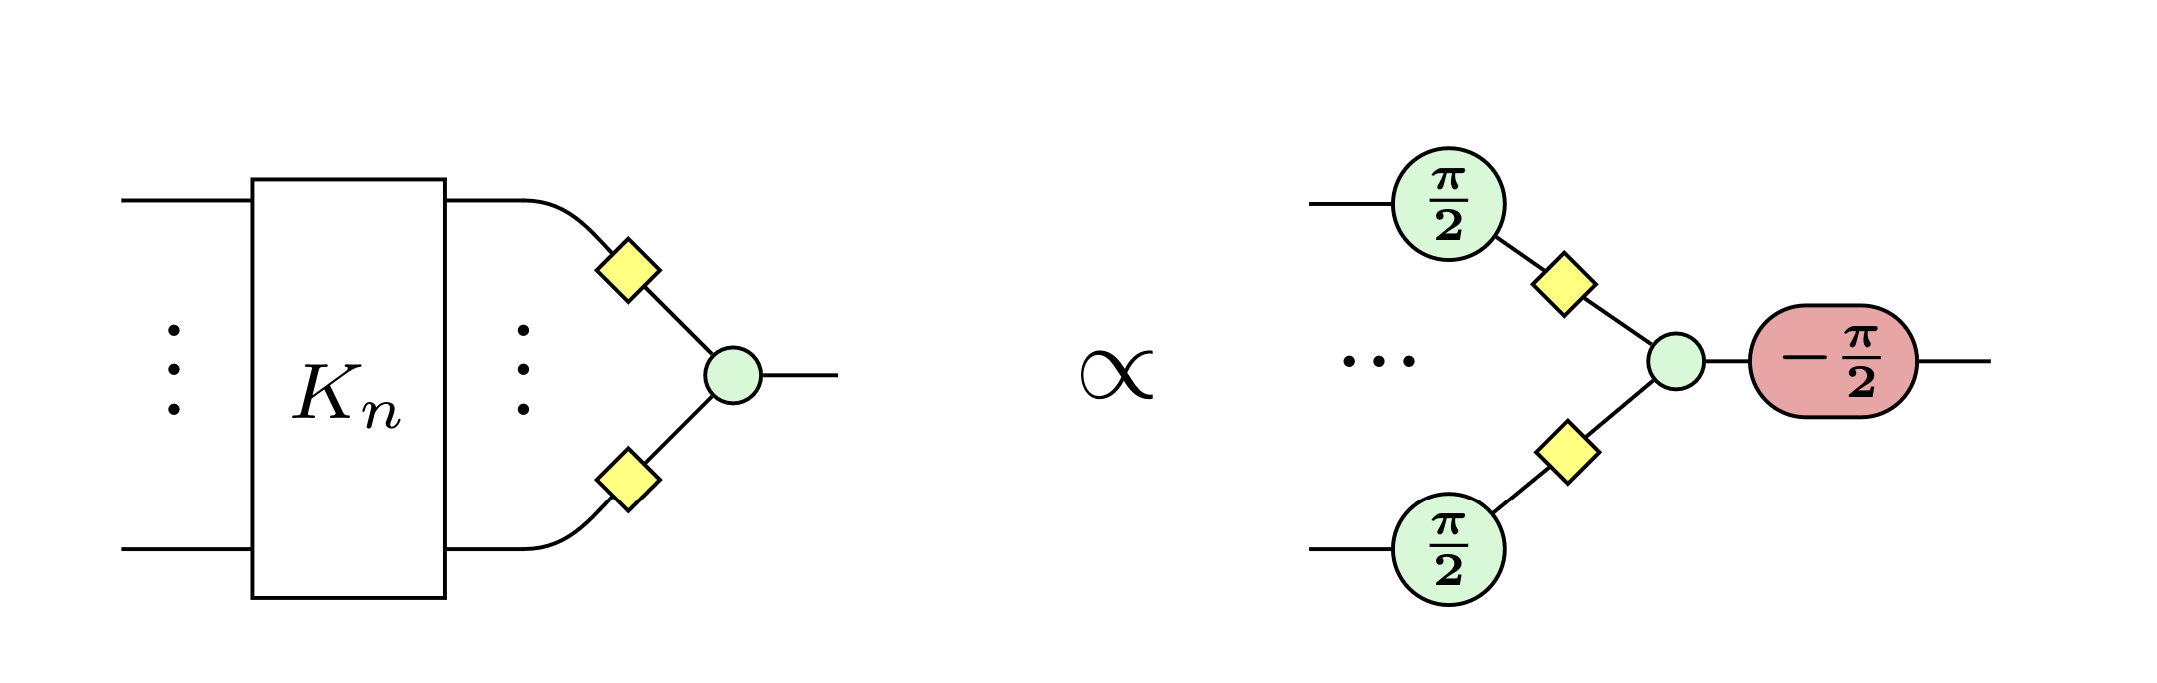
\includegraphics[width=0.8\linewidth]{./figures/k_m_local_complementation.png}
	\caption{The $K_{m}$ local complementation.}
	\label{fig:k_m_local_complementation}
\end{figure}
\end{lemma}\label{lem:k_m_local_complementation}

The proof is by induction on $m$ and using lemma \ref{lem:k3_local_complementation} as the base case. 
The readers are referred to lemma 5.2.4 of \cite{KissingerWetering2024Book} for the detailed proof.

Using lemma \ref{lem:k_m_local_complementation}, we can prove the general local complementation identity, which will be important for our later discussion on tensor contraction algorithm.

Let us first define local complementation of a graph.

\begin{definition}[Local Complementation]
	The local complementation of a graph $G$ on a vertex $v$ is the operation that replaces the subgraph of $G$ induced by the neighbours of $v$ with its complement graph. 
	The resulting graph is denoted as $G*v$.
	Let $u, w$ be two neighbours of $v$ in $G$. $u$ is connected to $w$ in $G*v$ if and only if $u$ is not connected to $w$ in $G$. All other connections are left unchanged.
	An example of local complementation is shown in figure \ref{fig:local_complementation}.
\end{definition}

\begin{figure}[ht]
	\centering
    % Graph Board TikZ export
% Exported: 2026-08-10T08:02:48.532Z
% Title: Untitled Graph
% Nodes: 15, Edges: 20

\begingroup
% --- Colors (define-if-not-already-defined) ---
\providecolor{zxRed}{RGB}{232,165,165}   % X spiders
\providecolor{zxGreen}{RGB}{216,248,216} % Z spiders
\providecolor{zxYellow}{RGB}{255,255,0}     % hadamard 

\tikzset{
    EMPTY/.style={minimum size=3.4mm,
        outer sep=-1.7mm},
    DOT/.style={inner sep=0mm, minimum size=3.4mm, shape=circle,
        draw=black, outer sep=-0.5mm, line width=1pt},
    BLACK_DOT/.style={minimum size=1mm, inner sep=0.7mm,
        outer sep=-0.5mm, fill=black, shape=circle},
    WORD_BALL/.style={draw=black, shape=rectangle, minimum size=6.5mm,
        rounded corners=3.2mm, inner sep=1.2mm, outer sep=-1.0mm,
        scale=1, font={\large\boldmath}, line width=1pt},
    GREEN_DOT/.style={DOT, fill=zxGreen},
    GREEN_WORD_BALL/.style={WORD_BALL, fill=zxGreen},
    RED_DOT/.style={DOT, fill=zxRed},
    RED_WORD_BALL/.style={GREEN_WORD_BALL, fill=zxRed},
    YELLOW_BOX/.style={fill=zxYellow, draw=black, line width=1pt, shape=rectangle, inner sep=0.6mm,
        minimum height=3.4mm, minimum width=3.4mm,
        font={\large\boldmath}},
    EDGE/.style={draw=black, line width=1pt}
}
\pgfdeclarelayer{edgelayer}
\pgfdeclarelayer{nodelayer}
\pgfsetlayers{edgelayer,nodelayer,main}

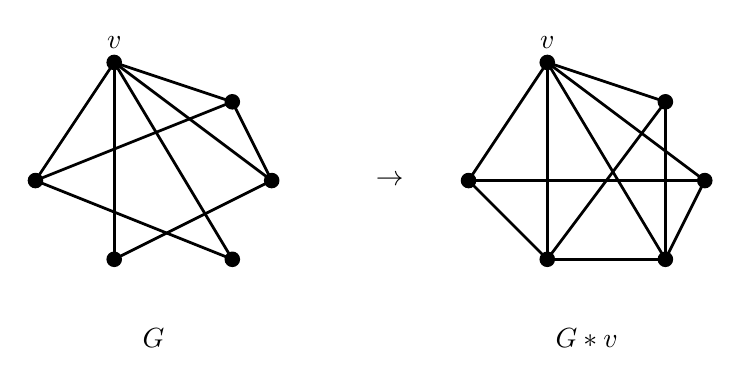
\begin{tikzpicture}
    \begin{pgfonlayer}{nodelayer}
        \node [label=above:{$v$}, BLACK_DOT] (1) at (-3.4, 1.7) {};
        \node [BLACK_DOT] (2) at (-4.4, 0.2) {};
        \node [BLACK_DOT] (3) at (-3.4, -0.8) {};
        \node [BLACK_DOT] (4) at (-1.9, -0.8) {};
        \node [BLACK_DOT] (5) at (-1.4, 0.2) {};
        \node [BLACK_DOT] (6) at (-1.9, 1.2) {};
        \node [label=above:{$v$}, BLACK_DOT] (7) at (2.1, 1.7) {};
        \node [BLACK_DOT] (8) at (1.1, 0.2) {};
        \node [BLACK_DOT] (9) at (2.1, -0.8) {};
        \node [BLACK_DOT] (10) at (3.6, -0.8) {};
        \node [BLACK_DOT] (11) at (4.1, 0.2) {};
        \node [BLACK_DOT] (12) at (3.6, 1.2) {};
        \node [EMPTY] (13) at (0.1, 0.2) {$\rightarrow$};
        \node [EMPTY] (14) at (-2.9, -1.8) {$G$};
        \node [EMPTY] (15) at (2.6, -1.8) {$G * v$};
    \end{pgfonlayer}
    \begin{pgfonlayer}{edgelayer}
        \draw[EDGE] (2) to (1);
        \draw[EDGE] (3) to (1);
        \draw[EDGE] (4) to (1);
        \draw[EDGE] (5) to (1);
        \draw[EDGE] (6) to (1);
        \draw[EDGE] (2) to (4);
        \draw[EDGE] (3) to (5);
        \draw[EDGE] (6) to (2);
        \draw[EDGE] (8) to (7);
        \draw[EDGE] (9) to (7);
        \draw[EDGE] (10) to (7);
        \draw[EDGE] (11) to (7);
        \draw[EDGE] (12) to (7);
        \draw[EDGE] (8) to (9);
        \draw[EDGE] (9) to (10);
        \draw[EDGE] (10) to (11);
        \draw[EDGE] (11) to (8);
        \draw[EDGE] (12) to (9);
        \draw[EDGE] (12) to (10);
        \draw[EDGE] (6) to (5);
    \end{pgfonlayer}
\end{tikzpicture}

\endgroup

	\caption{Local complementation of the graph $G$ on the vertex $v$. The subgraph induced by the neighbours of $v$ is replaced with its complement graph.}
	\label{fig:local_complementation}
\end{figure}

\begin{theorem}[Local Complementation Identity]
	Let $G$ be a ZX diagram consisting of $z$-spiders connected by Hadamard gates, and let $v$ be a vertex in $G$. 
	This $ZX$ diagram is equivalent up to a global constant to the ZX diagram of the local complementation of $G$ on $v$, denoted as $G*v$, up to some local unitaries applied to $v$ and its neighbours.
	See figure \ref{fig:local_complementation_identity}.
\end{theorem}

The concept of local complementation was introduced in \cite{Duncan_2020}, and is discussed in detail in the textbook \cite{KissingerWetering2024Book}.

\begin{figure}[ht]
	\centering
	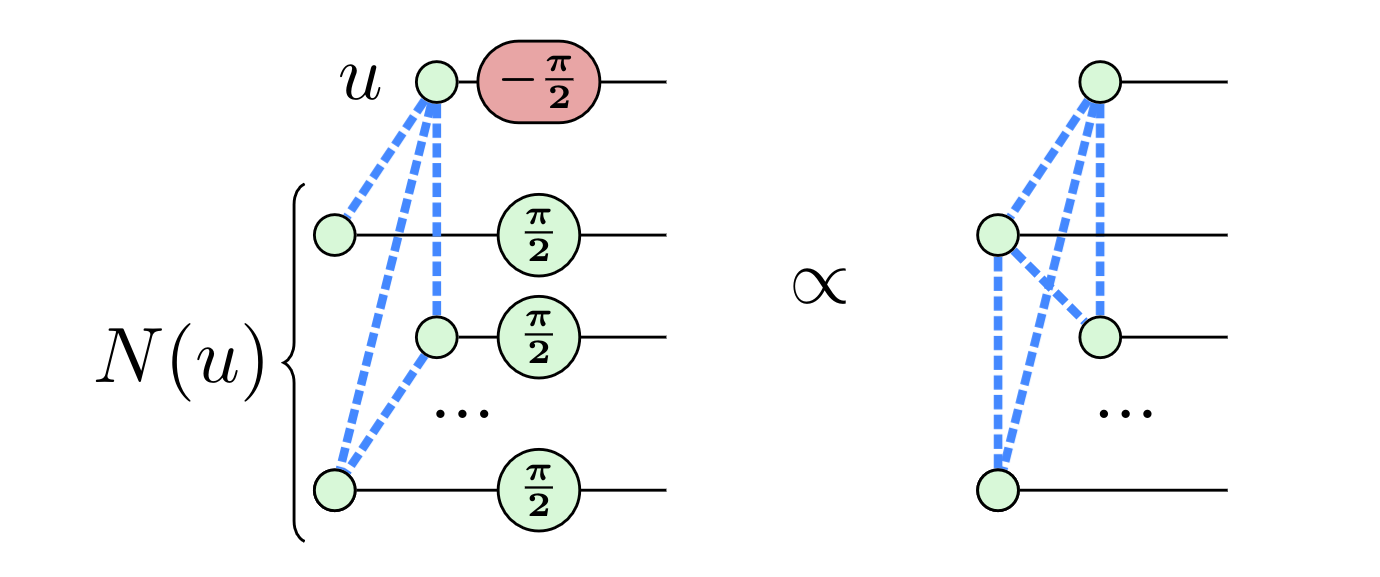
\includegraphics[width=0.8\linewidth]{./figures/general_local_complementation.png}
	\caption{General Local complementation identity. The ZX diagram of the local complementation of $G$ on $v$ is equivalent to the original ZX diagram up to a global constant and some local unitaries applied to $v$ and its neighbours.}
	\label{fig:local_complementation_identity}
\end{figure}
